\documentclass[oneside,11pt,openright]{report}

\usepackage[latin1]{inputenc}
\usepackage[american]{babel}
\usepackage{a4}
\usepackage{latexsym}
\usepackage{amssymb}
\usepackage{amsmath}
\usepackage{epsfig}
\usepackage[T1]{fontenc}
\usepackage{lmodern}
\usepackage[labeled]{multibib}
\usepackage{color}
\usepackage{datetime}
\usepackage{epstopdf} 
\usepackage{graphicx}
\usepackage{pgfplots}
\usepackage{caption}

\usepackage{pgf,tikz}
\usepackage{comment}
\usetikzlibrary{arrows,automata}
\usetikzlibrary{backgrounds,fit}
\usetikzlibrary{shapes,patterns}
\usetikzlibrary{calc,chains,positioning}

\renewcommand*\ttdefault{txtt}
\newcommand{\BigO}[1]{\ensuremath{\operatorname{O}\left(#1\right)}}
\newcommand{\BigT}[1]{\ensuremath{\Theta\left(#1\right)}}
\newcommand{\specialcell}[2][c]{%
  \begin{tabular}[#1]{@{}c@{}}#2\end{tabular}}
% see http://imf.au.dk/system/latex/bog/

\newcommand{\adjustimg}{% Horizontal adjustment of image
  \ifodd\value{page}\hspace*{\dimexpr\evensidemargin-\oddsidemargin}\else\hspace*{-\dimexpr\evensidemargin-\oddsidemargin}\fi%
}
\newcommand{\centerimg}[2][width=\textwidth]{% Center an image
  \makebox[\textwidth]{\adjustimg\includegraphics[#1]{#2}}%
}
\newcommand{\MakeHeap}{\textsc{MakeHeap}}
\newcommand{\FindMin}{\textsc{FindMin}}
\newcommand{\Insert}{\textsc{Insert}}
\newcommand{\DeleteMin}{\textsc{DeleteMin}}
\newcommand{\DecreaseKey}{\textsc{DecreaseKey}}
\newcommand{\Delete}{\textsc{Delete}}
\newcommand{\Meld}{\textsc{Meld}}
\newcommand{\Dijkstra}{\textsc{Dijkstra}}
\newcommand{\NULL}{\textbf{null}}

\begin{document}

%%%%%%%%%%%%%%%%%%%%%%%%%%%%%%%%%%%%%%%%%%%%%%%%%%%%%%%%%%%%%%%%%%%%%%%

\pagestyle{empty} 
\pagenumbering{roman} 
\vspace*{\fill}\noindent{\rule{\linewidth}{1mm}\\[4ex]
{\Huge\sf Binary Heaps, Fibonacci Heaps and\\[2ex]Dijkstras shortest path}\\[4ex]
{\huge\sf Kristoffer Just Andersen, 20051234\\[2ex]
\huge\sf Troels Leth Jensen, 20051234 \\[2ex]
\huge\sf Morten Krogh-Jespersen, 20022362}\\[2ex]
\noindent\rule{\linewidth}{1mm}\\[4ex]
\noindent{\Large\sf Project 1, Advanced Data Structures 2013, Computer Science\\[1ex] 
\monthname\ \the\year  \\[1ex] Advisor: Gerth Stølting Brodal\\[15ex]}\\[\fill]}
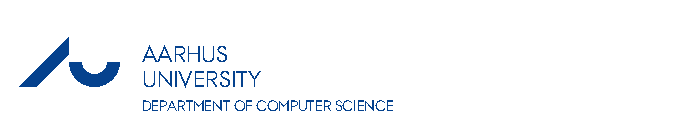
\epsfig{file=logo.eps}\clearpage

%%%%%%%%%%%%%%%%%%%%%%%%%%%%%%%%%%%%%%%%%%%%%%%%%%%%%%%%%%%%%%%%%%%%%%%

\tableofcontents
\pagenumbering{arabic}
\setcounter{secnumdepth}{2}

%%%%%%%%%%%%%%%%%%%%%%%%%%%%%%%%%%%%%%%%%%%%%%%%%%%%%%%%%%%%%%%%%%%%%%%

\chapter{Introduction}

needs content

\chapter{Binary heaps}

needs content

\section{Binary heap with array}

needs content

\section{Implementing decrease key}

needs content

\section{Time-complexity for binary heap with array}

\section{Binary heap with pointers}

needs content

\section{Implementing decrease key}

needs content

\section{Time-complexity for binary heap with pointers}

\section{Testing correctness of Binary Heaps}

needs content

\chapter{Fibonacci heaps}

In this chapter we focus on Fibonacci heaps, which is a data structure that has a forest of rooted trees as opposed to a binary heap that only has one tree \cite{FT87}. The data structure was invented by Michael L. Fredman and Robert Endre Tarjan and was published in the Journal of ACM in 1987. It has it name because the size of any subtree in a Fibonacci heap will be lower bounded by $F_{k+2}$ where $k$ is the degree of the root in that subtree and $F_k$ is the kth Fibonacci number. Below is the time-complexities of each of the heap operations listed:

\begin{center}
  \begin{tabular}{ l | c | c | c }
    Operation & Binary heap & \specialcell{Fibonacci heap v1\\(amortized)} & \specialcell{Fibonacci heap v2\\(amortized)} \\ \hline
    \MakeHeap & $\BigT{1}$ & $\BigT{1}$ & $\BigT{1}$ \\ 
    \FindMin & $\BigT{1}$ & $\BigT{1}$ & $\BigO{l(\lg (\frac{n}{l}) + 1)}$\\ 
    \Insert & $\BigT{\lg n}$ & $\BigT{1}$ & $\BigT{1}$ \\ 
    \DeleteMin & $\BigT{\lg n}$ & $\BigO{\lg n}$ & $\BigT{1}$  \\ 
    \DecreaseKey & $\BigT{\lg n}$ & $\BigO{1}$ & $\BigO{1}$ \\ 
    \Delete & $\BigT{\lg n}$ & $\BigO{\lg n}$ & $\BigT{1}$ \\ 
    \Meld & $\BigT{n}$ & $\BigT{1}$ & $\BigT{1}$ \\
  \end{tabular}
\end{center}

\section{Properties of the Fibonacci heap}

The Fibonacci heap is a heap that has better amortized bounds than binary heaps, and one of the reasons to this is that some of the operations are lazy. We will later see that this has a big impact on worst-case time complexities for the operations that do the heavy lifting.

The heap maintains a collection of root nodes in a doubly linked circular list that supports inserting, joining and single deletions in constant time. Each node has a left and a right sibling pointer that facilitates the circular doubly linked list, a pointer to the parent and a pointer to an arbitrary child. If there is no parent or child the pointers point to \NULL. A node is marked if it has had a child removed. If a child is removed from a parent that is already marked the parent will be moved to the root and the parents parent will be marked or moved. A mark on a node is removed when it is added as a child to another node.

Items added to the heap are added as single-item trees rooted with a node for the corresponding item. It is only when performing a linking step that trees grow. Therefore, the degree of nodes can only change when linking, removing or decreasing the key of an item, since decreasing the key of an item cuts the node from its parent and move the node up to be joined with the roots. 

The upper bound $D(n)$ on the degree of any node of an n-node Fibonacci is $\BigO{\lg n}$~\cite[p.~523]{ITA09}~\cite[p.~604]{FT87}. This can be shown by first observing that the degree of any node $y$ in the Fibonacci heap is bounded by when it was inserted into the list of its parent $x$ childs, where $degree(x) = k$. When $y_i$ was linked to $x$, where $i$ declares when $y$ was added to the children list of $x$, $x$ and $y_i$ must have had the same degree which results in $degree(y_i) \le k - 1$. $y$ could have lost at most one child before it would be cut from $x$ resulting in $degree(y_i) \ge i - 2$ where $i = 1,2,\cdots,k$.

By three different induction proofs and the lemma described above, it can be shown that if $k = degree(x)$ for any node in a Fibonacci heap then $size(x) \ge F_{k+2} \ge \phi^k$, where $\phi = (1+\sqrt{5}) / 2$ also known as the golden ratio. Hereafter, showing the bound of $D(n)$ is straight forward:
\begin{gather*}
    n \ge size(x) \ge \phi^k \\
    \Downarrow \\
    k \le \lfloor \log_\phi n \rfloor    
\end{gather*}

\section{The potential method}

We will analyse the amortized running times of the Fibonacci heaps by using the potential function \cite[p.~215]{FT87}. A potential function maps a state of a data structure to a real number representing the potential contained in that data structure \cite[p.~459]{ITA09}. The amortized cost of an operation $c_i$ that transforms a data structure in state $D_{i-1}$ to $D_{i}$ is:
\begin{align*}
    \hat{c} = c_i + \Phi(D_i) - \Phi(D_{i-1})
\end{align*}
The amortized cost is therefore the cost of the operation $c_i$ plus the change in the potential. If the operation releases potential, the relased potential gets subtracted from the cost of the operation. For the Fibonacci heaps we define the potential function as:

\begin{align*}
    \Phi(H) = trees(H) + 2marked(H)
\end{align*}

Where trees define the number of trees/roots in the forest and marked is the number of marked nodes. The reason to why marked nodes contains two units of potential is that one unit pays for the cut and the other pays for the node to become a root and thereby form a new tree.

\section{Fibonacci heap version 1}

The first Fibonacci heap variant we present is the original version proposed in FT87. A potential function is used to analyze the perfomance, thus the above stated time-complexities are amortized.

Our implementation pretty much follows from the article, with few minor exceptions. The article do not specify exactly how a node is found from an item in constant time, so we decided to place a pointer on the item. Also, melding is not totally destructable since we join the heap in of the two existing heaps and return an arbitrary one. 

The article mentions that $\Delete$ takes $\BigO{1}$ if the node to remove is not the min-node and without cascading deletes. The children of the node to delete must be moved up onto the root which can only be done in constant time if every children has a pointer to a parent pointer. In this way, we only have to change one pointer to update all parent pointers for the children of the beforementioned node. Since the running time of the \Delete~operation is amortized $\BigO{\lg n}$ we chose a simpler version where we just update all parent pointers one by one. As stated above $size(node) \le \BigO{\lg n}$ so this only takes $\BigT{\lg n}$ time.

\MakeHeap~constructs a new empty Fibonacci heap, which means there are not roots and no marked nodes. Therefore, the potential of the empty heap is 0 and constructing the heap can be done in constant time. \FindMin~does not alter the potential and is only a pointer lookup which clearly is also a constant time operation. \Insert~inserts a new root which increments the potential by one. Combine that with the actual cost which is $\BigO{1}$ the \Insert~operation is $\BigO{1}$. \Meld~can be carried out in $\BigO{1}$ actual time and since the change is:
\begin{align*}
    \Delta & = \Phi(H) - (\Phi(H_1) + \Phi(H_2)) = 0
\end{align*}
the \Meld~operation has time $\BigO{1}$.

When analyzing the amortized cost of $\DeleteMin$, let us say that the minimum node to delete is actually the node with degree $D(n)$ which is the upper bound on the maximum degree for any node. Setting the parent pointer to \NULL and concatinating each node with the root list takes constant time for each of the $D(n)$ children. 
The linking phase work on at most $D(n) + tress(H) - 1$ trees, since we have removed the minimum node from the root list and at most will be adding $D(n)$. We also join trees of same degree, but when two trees are joined only one will remain in the root list, so this can happen at most the number of roots in the root list. Therefore, the actual working time is $\BigO{D(n) + trees(H)}$.

The potential before the $\DeleteMin$ operation executues is $trees(H) + 2marked(H)$. After, at most $D(n) + 1$ roots will exist because all others would be removed during the linking phase and there is no change to marked nodes. Therefore, we have that:
\begin{align*}
    \DeleteMin & = \BigO{D(n) + trees(H)} + \left(\left(D(n) + 1\right) + 2marked(H)\right) \\
    & - \left(trees(H) + 2marked(H)\right) \\
    & = \BigO{D(n)} + \BigO{trees(H)} - trees(H) \\
    & = \BigO{D(n)}
\end{align*}
Actually, a slight subtlety is happening above. We can turn up the units that we pay to cover the hidden constant in $\BigO{trees(H)}$, which allows us to cancel those two terms out, resulting in an amortized running time of $\BigO{D(n)} \le \BigO{\lg n}$.

$\DecreaseKey$ takes constant time for moving the node for the item with the decreased key to the root, but then $c$ cascading deletes can occur. Therefore, the actual time is $\BigO{c}$. The change is potential is:
\begin{align*}
    \Delta & = \BigO{trees(H) + (c - 1) + 1} + 2(marked(H) - (c-1) + 1) \\
    &- (trees(H) + 2marked(H) \\
    & = \BigO{trees(H) + c} + 2(marked(H) - c + 2) - (trees(H) + 2marked(H)) \\
    & = 4 - c
\end{align*}
Therefore, the amortized running time of $\DecreaseKey$ is $\BigO{c} + 4 - c = \BigO{1}$

Last, we have to cover the running time of $\Delete$. First, we cut the node and move the children to the root, which is at most $D(n)$ operations. Next, a chain of cascading deletes can occur where the length is $c$, making the actual time $\BigO{D(n) + c}$. The change in potential is as follows:
\begin{align*}
    \Delta & = \BigO{trees(H) + D(n) + c} + 2(marked(H) - c + 2) \\
    &- (trees(H) + 2marked(H) \\
    & = D(n) + 4 - c \\
\end{align*}
But as we showed for $\DecreaseKey$, the released potential pays for the cascading deletes, so we only have to pay the $D(n)$ for the actual time and $D(n)$ for the change in potential, which is $\BigO{D(n)} \le \BigO{\lg n}$.

\section{Worst case time-complexity for Fib heap v1}

There are three operations where changes to the potential occurs, and thus, the stated times are amortized for $\DeleteMin$, $\DecreaseKey$ and $\Delete$. Below we illustrate the worst-case for each of these operations by showing a configuration and how that configuration can be obtained from a sequence of operations :

\subsection{Worst case time-complexity for $\DeleteMin$}

As we showed in the previous section the actual time for performing $\DeleteMin$ is $\BigO{D(n) + trees(H)}$. When linking trees the change in potential pays for $trees(H)$, therefore, it is in the amount of trees the worst case configuration for $\DeleteMin$ can be found. It is easy to see that the worst case is when all the nodes in the heap is at the root in a linked list:

\begin{center}
  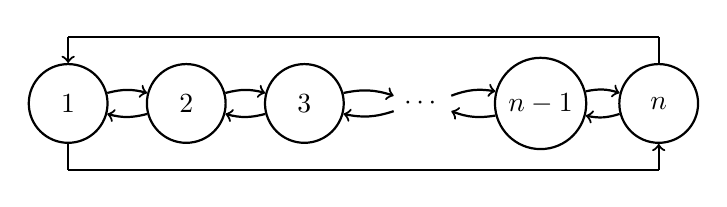
\begin{tikzpicture}[thick,->,auto,node distance=1.5cm]
    \tikzstyle{state}=[circle, minimum size=1cm, draw]
  
    \node[state]          (1) {1};
    \node[state]         (2) [right of=1] {2};
    \node[state]         (3) [right of=2] {3};
    \node          (dots) [right of=3] {$\cdots$};
    \node[state]         (nminusone) [right of=dots] {$n-1$};
    \node[state]         (n) [right of=nminusone] {$n$};
    \node          (dummy1) [below=0.2cm of 1] {};
    \node          (dummy2) [below=0.2cm of n] {};
    \node          (dummy3) [above=0.2cm of 1] {};
    \node          (dummy4) [above=0.2cm of n] {};
    
    \path (1)   edge [bend left=15] (2);
    \path (2) edge [bend left=15] (1);
    \path (2) edge [bend left=15] (3);
    \path (3) edge [bend left=15] (2);
    \path (3) edge [bend left=15] (dots);
    \path (dots) edge [bend left=15] (3);
    \path (dots) edge [bend left=15] (nminusone);
    \path (nminusone) edge [bend left=15] (dots);
    \path (nminusone) edge [bend left=15] (n);
    \path (n) edge [bend left=15] (nminusone);
    \path[-] (1) edge (dummy1.center);
    \path[-] (dummy1.center) edge (dummy2.center);
    \path (dummy2.center) edge (n);
    \path[-] (n) edge (dummy4.center);
    \path[-] (dummy4.center) edge (dummy3.center);
    \path (dummy3.center) edge (1);
  \end{tikzpicture}
\end{center}

This configuration can be achieved by just calling insert $n$ times. For simplicity, let us assume that $n$ is odd, and a call to $\DeleteMin$ happens. In the above example 1 will be removed and we are left with $n-1$ root nodes to link. This results in $n-1$ key comparisons, but all the trees of rank 1 will be joined too and this will continue until no trees of duplicate size is found.
\begin{align*}
  \text{\# of operations} = \BigO{n-1} + \BigO{\frac{n-1}{2}} + \BigO{\frac{n-1}{2^2}} + \cdots + \BigO{\frac{n-1}{2^{\lg (n-1)-1}}}
\end{align*}
which is $\BigT{n}$.

\subsection{Worst case time-complexity for $\Delete$ and $\DecreaseKey$}

As we shoved in the previous section, the release in potential for cascading deletes pays for most of the work, therefore, we can find a worst-case configuration that will perform considerably worse in actual time.

If $\Delete$ is invoked with the min-node as argument then $\Delete$ calls $\DeleteMin$, therefore, the worst case for $\Delete$ is $\BigT{n}$, but we will show that without the min-node as argument, we still end up with $\BigT{n}$. The following observation holds true for $\DecreaseKey$ as well.

If we delete a child to an arbitrary node $x$ we mark $x$ if is not marked and if it is marked, we cut $x$ from its parent, move the subtree formed by $x$ to the root and try to mark the previous parent of $x$. This could result in cascading deletes. Therefore, the worst situation would be the following configuration:
\begin{center}
  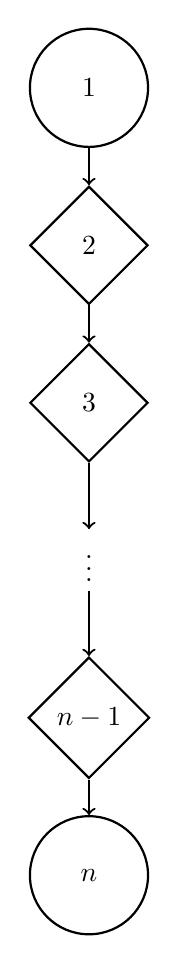
\begin{tikzpicture}[thick,->,auto,node distance=2cm]
    \tikzstyle{node}=[circle, minimum size=1.5cm, draw]
    \tikzstyle{marked}=[diamond, minimum size=1.5cm, draw]
  
    \node[node]    	  (1) {1};
    \node[marked]         (2) [below of=1] {2};
    \node[marked]         (3) [below of=2] {3};
    \node          (dots) [below of=3] {$\vdots$};
    \node[marked]         (nminusone) [below of=dots] {$n-1$};
    \node[node]         (n) [below of=nminusone] {$n$};
    
    \path (1) edge (2);
    \path (2) edge (3);
    \path (3) edge (dots);
    \path (dots) edge (nminusone);
    \path (nminusone) edge (n);

  \end{tikzpicture}
\end{center}

where a diamond is modelling a marked node. If either $\DecreaseKey$ or $\Delete$ is called with an item corresponding to node $n$ a cascading delete will begin and will not stop until it reaches $2$ in this example. The amount of operations is therefore the entire chain:
\begin{align*}
  \text{length of chain} = n - 1
\end{align*}
which is $\BigT{n}$.

Such a configuration can be obtained by calling $\Insert$ with two very high numbers $x$ and $y$ and one smaller and call $\DeleteMin$:

\begin{center}
  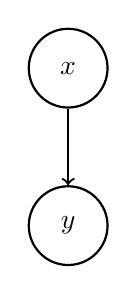
\begin{tikzpicture}[thick,->,auto,node distance=2cm]
    \tikzstyle{node}=[circle, minimum size=1cm, draw]
    \tikzstyle{marked}=[diamond, minimum size=1cm, draw]
  
    \node[node]    	  (1) {$x$};
    \node[node]           (2) [below of=1] {$y$};
    
    \path (1) edge (2);

  \end{tikzpicture}
\end{center}

If we insert three new items $x'$, $y'$ $z$ with keys slightly smaller where $z$ is the smallest key we will have the following forest:

\begin{center}
  \begin{tikzpicture}[thick,->,auto,node distance=2cm]
    \tikzstyle{node}=[circle, minimum size=1cm, draw]
  
    \node[node]    	  (x) {$x$};
    \node[node]           (y) [below of=x] {$y$};
    \node[node]    	  (x') [right of=x] {$x'$};
    \node[node]    	  (y') [right of=x'] {$y'$}; 
    \node[node]    	  (z) [right of=y'] {$z$};
   
    \path (1) edge (2);

  \end{tikzpicture}
\end{center}

If we call $\DeleteMin$, call $\Delete$ on $y'$ and call insert with three new items as above, we can get the following configuration:

\begin{center}
  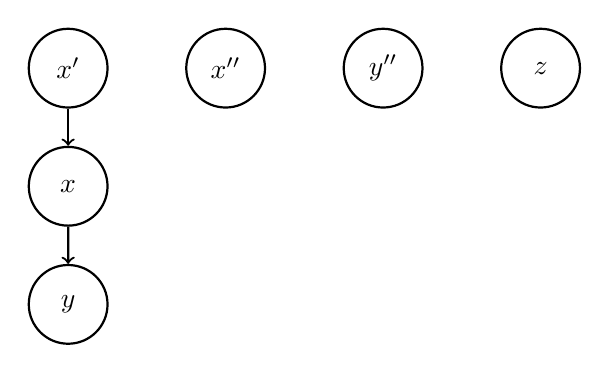
\begin{tikzpicture}[thick,->,auto,node distance=2cm]
    \tikzstyle{node}=[circle, minimum size=1cm, draw]
  
    \node[node]    	  (x') {$x'$}
    child{node[node]      (x) {$x$}
      child{node[node]    (y) {$y$}}};
    \node[node]    	  (x'') [right of=x'] {$x''$};
    \node[node]    	  (y'') [right of=x''] {$y''$}; 
    \node[node]    	  (z) [right of=y''] {$z$};
   
  \end{tikzpicture}
\end{center}
where $z$ again is the smallest key. $\DeleteMin$ gives:

\begin{center}
  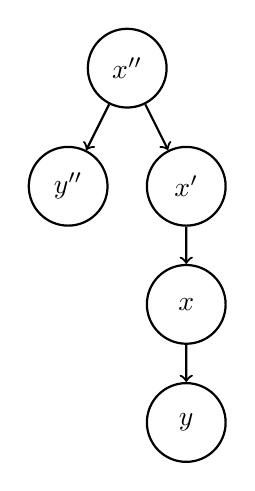
\begin{tikzpicture}[thick,->,auto,node distance=2cm]
    \tikzstyle{node}=[circle, minimum size=1cm, draw]
  
    \node[node]    	  (x'') {$x''$}
    child{node[node]      (y'') {$y''$}}
    child{node[node]      (x') {$x'$}
      child{node[node]    (x) {$x$}
        child{node[node]  (y) {$y$}}}};
   
  \end{tikzpicture}
\end{center}
where $\Delete$ with $y''$ as argument will result in a chain. By using this approach we can easily build up a single chain of height $n$.

\section{Fibonacci heap version 2}

In this second version of a Fibonacci heap we try to be more lazy, by doing as little work as possible for $\Delete$ and $\DeleteMin$. When a call to either one of the operations is called, we mark the node as vacant but then halt to do any additional work. This makes $\Delete$ and $\DeleteMin$ run in $\BigO{1}$.

We have to do some work at one point which happens in $\FindMin$. Now, $\FindMin$ works like $\DeleteMin$ in version 1, but also has to delete every vacant node it meets on the path. $\Meld$ also requires little work, such that when melding two heaps, if a root is marked as vacant it should be the new root of the resulting heap. There is no change in actual time for $\Meld$.

Below is an image from our test-framwork showing how a tree looks like with vacant nodes:

\mbox{} \par
\noindent\centerimg{delete_39}
After a call to $\FindMin$ thee heap looks like:

\mbox{} \par
\noindent\centerimg{find_min}

Let us analyze the time for the $\FindMin$ operation. Let $l$ mark the number of vacant nodes. If $l=0$ then $\FindMin$ points to the node representing the item with the minimum key, and the work is constant. If $l \ge 1$ then the amortized running time is the new roots created from destroying vacant nodes and moving the non-vacant child nodes to the root plus the linking of the trees which is at most $\BigO{\lg n}$. We argued previously that a node $y$ have $degree(y_i) \ge i - 2$ for $i = 1,2,\cdots,k$ where $k$ is the degree of its parent. We use this to say that at least one of the vacant nodes will have a rank of $k-2$. We also know that the size of subtree rootet at a node with degree $k-2$ will be at least be of size $\phi^{k-2}$. If all children of the vacant nodes we destroy are nonvacant, they will increase the number of trees and thereby the potential by:
\begin{align*}
\sum_{i=1}^l \phi^{k_j-2} \le n
 \end{align*}
where $k_1, k_2,\cdots,k_i$ are nonvacant nodes. The sum is maximized for $k_i$. MAYBE SOME MORE??

\section{Worst case time-complexity for Fib heap v2}

The worst case example is extremely easy. Since $l$ and $n$ are disjoint, the can be filled with vacant nodes. The worst-case would then be calling $\FindMin$, just to find out that no such node exist. 

\section{Testing correctness of Fibonacci Heaps}

Implementing the Fibonacci heaps in C required a lot of work and since we are working with that many pointers, we decided very early in the proces that we needed some kind of test-framework to assist us. 

First, we implemented a consistency checker, that checks the following properties for each node $x$: That the nodes the sibling pointers of $x$ points to points to $x$ with the corresponding sibling pointer. That the parent pointer is correct if the node $x$ is a child of any node and that the key is larger than its parent. Still, this tests the implementation more than the properties of the Fibonacci heaps, so we needed one more tool.

We build a pretty printer that could convert any subtree (or heap) to a graphical representation, such that we could see how the heap looked like. We then made test-cases, that for each operation printed the output, and then we could manually check if $\DeleteMin$, $\Delete$ and $\DecreaseKey$ behaved as it should. We manually checked test-instances of size less than or equal to 100 operations.

Attached in the zipped-file companying the report are generated images we have used to check correctness.

Lastly, since we now have four datastructures, we could check the output for each and compare it with the others, to make sure, that all our heaps answer correctly (or all could answer wrong the same way, which is highly unlikely).

\chapter{Test-results}

needs content

\chapter{\Dijkstra's algorithm}

\Dijkstra's~algorithm is an graph search algorithm that computes that solves the single-source shortest path problem. Without a min-priority queue the algorithm runs in $\BigO{V^2} \ge \BigO{E}$ for a graph $G=(V, E)$[3]. But we have two heaps that can actually be used as priority queues, so this will give us better asymptotic running times depending on the connectivity of the graph.
Normally, $\Dijkstra$ is implemented by using the $\DecreaseKey$ operation, but if we disregard space, we can actually implement $\Dijkstra$ without $\DecreaseKey$ and just insert new nodes every time we find a shorter path. Below is a summery of the running time and space complexities:

\begin{center}
  \begin{tabular}{ l | c | c | c}
    $\Dijkstra$ & Binary heaps & Fibonacci heap v1 & Fibonacci heap v2 \\ \hline
    with & $\BigO{(n+m)\lg n}$ & $\BigO{n\lg n + m}$ & $\BigO{n\lg n + m}$ \\
    without & $\BigO{(n+m)\lg n}$ & $\BigO{n\lg n + m}$ & $\BigO{n\lg n + m}$ \\     
  \end{tabular}
\end{center}

We represent graphs with an by a linked list so running $\Dijkstra$ with inserts will make a drastic increase in memory consumption for sparsely connected graphs, but only be a constant factor larger for a fully connected graph.

\section{Running times for $\Dijkstra$ with heaps}

We can show an upper bound on the time complexity for $\Dijkstra$ as a function taking the number of nodes $n=|V|$ and the numbers of edges $m=|E|$ as such: $\BigO{n \cdot dm + m \cdot dk}$ where $dm$ denotes the number of $\DeleteMin$ operations and $dk$ denotes the number of $\DecreaseKey$ operations.

First, let us consider Binary heaps and the case for $\Dijkstra$ with $\DecreaseKey$ operations. A node can never be readded once it has been deleted by $\DeleteMin$, therefore there can only be $n$ $dm$ operations. For each node, there can be up to $m$ $dk$ operations, one for each adjacent node in the graph. Since $\Insert$, $\DeleteMin$ and $\DecreaseKey$ all take logarithmic time, the total time is $\BigO{(n+m)\lg n}$. For the $\Dijkstra$ version with $\Insert$s only, the $m$ previus calls to $\DecreaseKey$ will now call $\Insert$ instead but the time will remain the same.

We are able to reduce the time complexity asymptotically when we use a Fibonacci heap. For Fibonacci heaps, $\DecreaseKey $ takes amortized time $\BigO{1}$ and $\DeleteMin$ takes amortized time $\BigO{\lg n}$ resulting in the time-complexity $\BigO{m+n\lg n}$ for $\Dijkstra$ with Fibonacci heap version 1. Because the time-complexity for $\Insert$ is also $\BigO{1}$, using $\Dijkstra$ without $\DecreaseKey$ has the same total time complexity.

So what happens when we are lazy with deletions, and for $\DeleteMin$ mark a node as vacant in Fibonacci version 2? There are no random deletions in the Fibonacci heap when running $\Dijkstra$, therefore $l$, which denotes the number of vacant nodes, has an upper bound of $1$. Therefore, the amortized time for $\FindMin$ is $\BigO{\lg n + 1}$ which results in the same running times for $\Dijkstra$ as Fibonacci heap version 1.

\section{Connectivity and generating graphs}

Above we argued for the running times of the $\Dijkstra$ algorithms, and as we can see, the running times are dominated by the number of edges for the graph. This suggest, that sparsely connected graphs can run quicker than highly connected graphs.

If the graph is sufficiently sparse it is an effective speed-up to implement $\Dijkstra$ using a min-priority queue of some sort. For Binary heaps, the threshold is when $m = o(n^2 / \lg n)$:
\begin{align*}
    \BigO{(n+m)\lg n} = \BigO{(n^2/\lg n)\lg n} = \BigO{n^2}
\sum_{i=1}^l \phi^{k_j-2} \le n
 \end{align*}
 which is the same running time as without a min-priority queue.
 
For Fibonacci heaps the time $\BigO{n\lg n + m}$ suggest, since $m$ dominates $n \lg n$, that if the graphs is not totally connected the Fibonacci heap will run quicker or in the same time as $\Dijkstra$ without min-priority queues. We are very confident, that the graph should be stricly sparser since the running time in $\operatorname{O}$-notation for Fibonacci heaps hide away a very large constant.

Because connectivety is a factor when running $\Dijkstra$ we are, when testing the running times for the $\Dijkstra$ algorithms, generating graphs by supplying size and connectivity probability as parameters to our graph-creation program. This is based on the pseudo-random number generator in C but we will use the resulting graphs as if they were completely randomly generated graphs with an expected probality on the number of edges in the graph.

\section{Testing time-complexities for \Dijkstra}

Because we have four different heaps and two different implementations of $\Dijkstra$ we have a lot of test to perform. We are generating graphs in the interval from 100 to 20.000 and increments of 100 nodes. A graph with 20.000 nodes represented by an adjacency matrix where all indicies are int is by our calculation around 1.5 GB, which should give us enough information about running times for large graphs.

For each level in our node-size interval we have 10 different graph connectivity-probabilities, 10 \% to 100 \% in steps of 10 \%, where we do following three times: generate a random graph with beforementioned probability and size and run all heaps and dijkstra algorithms on this instance three times to find an average. Thus:
\begin{align*}
    \text{\# of tests} = 200 * 10 * 3 * 8 * 3 = 144.000 
 \end{align*}



\chapter{Binary heap vs Fibonacci heap}

needs content

\chapter{Test-results}


\begin{minipage}[c]{\textwidth}
\centering
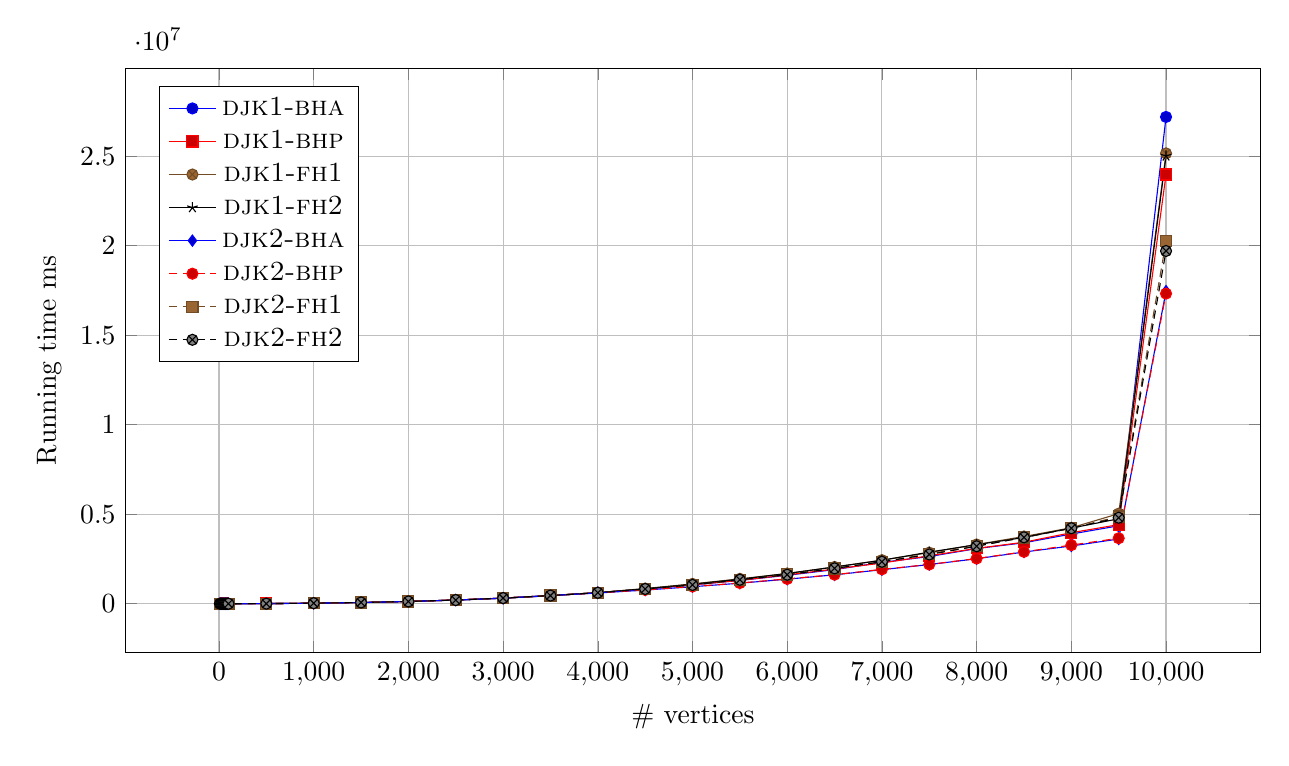
\begin{tikzpicture}
        \begin{axis}[
            xlabel = \# vertices,
            ylabel = Running time ms,
            height=9cm,
            width=16cm,
    		grid=major,
            xtick={0,1000,2000,...,10000},
            scaled x ticks = false,
            legend pos=north west
    	]
    		
    	\addplot coordinates {
(10,0)
(20,0)
(30,0)
(40,0)
(50,0)
(60,0)
(70,0)
(80,0)
(90,0)
(100,0)
(500,2222)
(1000,30000)
(1500,70000)
(2000,125555)
(2500,201111)
(3000,307777)
(3500,444444)
(4000,621111)
(4500,815555)
(5000,1051111)
(5500,1301111)
(6000,1588888)
(6500,1905555)
(7000,2310000)
(7500,2636666)
(8000,3081111)
(8500,3404444)
(9000,3893333)
(9500,4353333)
(10000,27196666)


    	};
        
    	\addlegendentry{\textsc{djk1-bha}}

                \addplot coordinates {
(10,0)
(20,0)
(30,0)
(40,0)
(50,0)
(60,0)
(70,0)
(80,0)
(90,0)
(100,0)
(500,7777)
(1000,30000)
(1500,70000)
(2000,124444)
(2500,206666)
(3000,313333)
(3500,455555)
(4000,618888)
(4500,820000)
(5000,1055555)
(5500,1304444)
(6000,1608888)
(6500,1937777)
(7000,2273333)
(7500,2677777)
(8000,3091111)
(8500,3435555)
(9000,3967777)
(9500,4416666)
(10000,23982222)

    	};
        
    	\addlegendentry{\textsc{djk1-bhp}}

        \addplot coordinates {
(10,0)
(20,0)
(30,0)
(40,0)
(50,0)
(60,0)
(70,0)
(80,0)
(90,0)
(100,0)
(500,8888)
(1000,28888)
(1500,68888)
(2000,126666)
(2500,204444)
(3000,311111)
(3500,447777)
(4000,617777)
(4500,848888)
(5000,1107777)
(5500,1390000)
(6000,1687777)
(6500,2053333)
(7000,2434444)
(7500,2854444)
(8000,3308888)
(8500,3756666)
(9000,4244444)
(9500,5031111)
(10000,25161111)

    	};
        
    	\addlegendentry{\textsc{djk1-fh1}}

        \addplot coordinates {
(10,0)
(20,0)
(30,0)
(40,0)
(50,0)
(60,0)
(70,0)
(80,0)
(90,0)
(100,0)
(500,6666)
(1000,30000)
(1500,66666)
(2000,125555)
(2500,207777)
(3000,311111)
(3500,454444)
(4000,620000)
(4500,836666)
(5000,1090000)
(5500,1370000)
(6000,1688888)
(6500,2052222)
(7000,2426666)
(7500,2883333)
(8000,3300000)
(8500,3700000)
(9000,4224444)
(9500,4746666)
(10000,25015555)

    	};
        
    	\addlegendentry{\textsc{djk1-fh2}}


        \addplot coordinates {
(10,0)
(20,0)
(30,0)
(40,0)
(50,0)
(60,0)
(70,0)
(80,0)
(90,0)
(100,0)
(500,8888)
(1000,27777)
(1500,66666)
(2000,126666)
(2500,206666)
(3000,311111)
(3500,461111)
(4000,597777)
(4500,762222)
(5000,948888)
(5500,1146666)
(6000,1370000)
(6500,1615555)
(7000,1901111)
(7500,2190000)
(8000,2511111)
(8500,2888888)
(9000,3225555)
(9500,3616666)
(10000,17464444)
        };
        
    	\addlegendentry{\textsc{djk2-bha}}

        \addplot coordinates {
(10,0)
(20,0)
(30,0)
(40,0)
(50,0)
(60,0)
(70,0)
(80,0)
(90,0)
(100,0)
(500,7777)
(1000,28888)
(1500,70000)
(2000,126666)
(2500,211111)
(3000,317777)
(3500,455555)
(4000,603333)
(4500,770000)
(5000,962222)
(5500,1156666)
(6000,1386666)
(6500,1623333)
(7000,1920000)
(7500,2192222)
(8000,2526666)
(8500,2900000)
(9000,3274444)
(9500,3657777)
(10000,17326666)
        };
        
        \addlegendentry{\textsc{djk2-bhp}}

        \addplot coordinates {
(10,0)
(20,0)
(30,0)
(40,0)
(50,0)
(60,0)
(70,0)
(80,0)
(90,0)
(100,0)
(500,6666)
(1000,28888)
(1500,70000)
(2000,127777)
(2500,207777)
(3000,310000)
(3500,463333)
(4000,621111)
(4500,813333)
(5000,1048888)
(5500,1327777)
(6000,1635555)
(6500,1967777)
(7000,2342222)
(7500,2792222)
(8000,3225555)
(8500,3702222)
(9000,4218888)
(9500,4871111)
(10000,20244444)
        };
        
        \addlegendentry{\textsc{djk2-fh1}}
        
        \addplot coordinates {
(10,0)
(20,0)
(30,0)
(40,0)
(50,0)
(60,0)
(70,0)
(80,0)
(90,0)
(100,0)
(500,4444)
(1000,30000)
(1500,70000)
(2000,126666)
(2500,205555)
(3000,314444)
(3500,455555)
(4000,612222)
(4500,824444)
(5000,1050000)
(5500,1340000)
(6000,1621111)
(6500,1975555)
(7000,2344444)
(7500,2751111)
(8000,3208888)
(8500,3708888)
(9000,4215555)
(9500,4804444)
(10000,19707777)
        };
        
        \addlegendentry{\textsc{djk2-fh2}}

        \end{axis}

    \end{tikzpicture}
    \captionof{figure}{Average time of running \textsc{Dijkstra1} and \textsc{Dijkstra2} on 100 \% connected graph}
    \label{fig:sample_figure}
\end{minipage}

\begin{minipage}[c]{\textwidth}
\centering
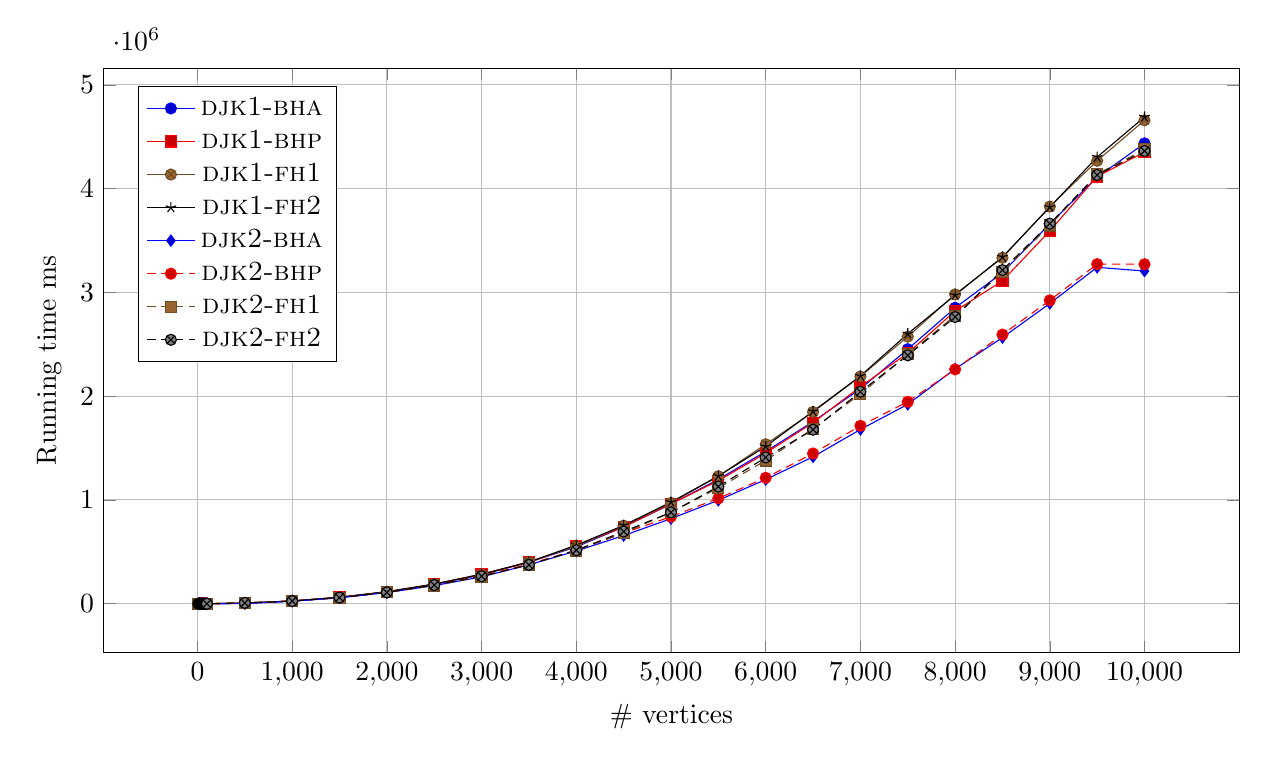
\begin{tikzpicture}
        \begin{axis}[
            xlabel = \# vertices,
            ylabel = Running time ms,
            height=9cm,
            width=16cm,
            grid=major,
            xtick={0,1000,2000,...,10000},
            scaled x ticks = false,
            legend pos=north west
    	]
    		
    		
    	\addplot coordinates {
(10,0)
(20,0)
(30,0)
(40,0)
(50,0)
(60,0)
(70,0)
(80,0)
(90,0)
(100,0)
(500,4444)
(1000,25555)
(1500,60000)
(2000,112222)
(2500,185555)
(3000,277777)
(3500,400000)
(4000,547777)
(4500,740000)
(5000,960000)
(5500,1197777)
(6000,1466666)
(6500,1754444)
(7000,2071111)
(7500,2452222)
(8000,2851111)
(8500,3188888)
(9000,3660000)
(9500,4110000)
(10000,4435555)

    
    	};
        
    	\addlegendentry{\textsc{djk1-bha}}

                \addplot coordinates {
(10,0)
(20,0)
(30,0)
(40,0)
(50,0)
(60,0)
(70,0)
(80,0)
(90,0)
(100,0)
(500,7777)
(1000,25555)
(1500,63333)
(2000,114444)
(2500,187777)
(3000,284444)
(3500,398888)
(4000,557777)
(4500,740000)
(5000,962222)
(5500,1185555)
(6000,1451111)
(6500,1744444)
(7000,2091111)
(7500,2414444)
(8000,2820000)
(8500,3111111)
(9000,3592222)
(9500,4116666)
(10000,4351111)


    	};
        
    	\addlegendentry{\textsc{djk1-bhp}}

        \addplot coordinates {
(10,0)
(20,0)
(30,0)
(40,0)
(50,0)
(60,0)
(70,0)
(80,0)
(90,0)
(100,0)
(500,7777)
(1000,26666)
(1500,62222)
(2000,114444)
(2500,187777)
(3000,282222)
(3500,403333)
(4000,554444)
(4500,752222)
(5000,971111)
(5500,1228888)
(6000,1536666)
(6500,1847777)
(7000,2190000)
(7500,2573333)
(8000,2981111)
(8500,3333333)
(9000,3826666)
(9500,4267777)
(10000,4657777)

    	};
        
    	\addlegendentry{\textsc{djk1-fh1}}

        \addplot coordinates {
(10,0)
(20,0)
(30,0)
(40,0)
(50,0)
(60,0)
(70,0)
(80,0)
(90,0)
(100,0)
(500,4444)
(1000,26666)
(1500,62222)
(2000,116666)
(2500,190000)
(3000,284444)
(3500,402222)
(4000,564444)
(4500,754444)
(5000,978888)
(5500,1230000)
(6000,1515555)
(6500,1853333)
(7000,2194444)
(7500,2601111)
(8000,2973333)
(8500,3341111)
(9000,3821111)
(9500,4303333)
(10000,4690000)

    	};
        
    	\addlegendentry{\textsc{djk1-fh2}}


        \addplot coordinates {
(10,0)
(20,0)
(30,0)
(40,0)
(50,0)
(60,0)
(70,0)
(80,0)
(90,0)
(100,0)
(500,2222)
(1000,24444)
(1500,56666)
(2000,107777)
(2500,174444)
(3000,258888)
(3500,375555)
(4000,507777)
(4500,656666)
(5000,820000)
(5500,996666)
(6000,1196666)
(6500,1415555)
(7000,1678888)
(7500,1921111)
(8000,2262222)
(8500,2564444)
(9000,2893333)
(9500,3241111)
(10000,3205555)
        };
        
    	\addlegendentry{\textsc{djk2-bha}}

        \addplot coordinates {
(10,0)
(20,0)
(30,0)
(40,0)
(50,0)
(60,0)
(70,0)
(80,0)
(90,0)
(100,0)
(500,6666)
(1000,27777)
(1500,58888)
(2000,110000)
(2500,181111)
(3000,268888)
(3500,382222)
(4000,515555)
(4500,681111)
(5000,838888)
(5500,1015555)
(6000,1213333)
(6500,1447777)
(7000,1714444)
(7500,1945555)
(8000,2257777)
(8500,2593333)
(9000,2923333)
(9500,3272222)
(10000,3271111)
        };
        
        \addlegendentry{\textsc{djk2-bhp}}

        \addplot coordinates {
(10,0)
(20,0)
(30,0)
(40,0)
(50,0)
(60,0)
(70,0)
(80,0)
(90,0)
(100,0)
(500,8888)
(1000,26666)
(1500,58888)
(2000,110000)
(2500,175555)
(3000,261111)
(3500,377777)
(4000,513333)
(4500,681111)
(5000,881111)
(5500,1115555)
(6000,1380000)
(6500,1686666)
(7000,2020000)
(7500,2402222)
(8000,2775555)
(8500,3197777)
(9000,3644444)
(9500,4140000)
(10000,4376666)
        };
        
        \addlegendentry{\textsc{djk2-fh1}}
        
        \addplot coordinates {
(10,0)
(20,0)
(30,0)
(40,0)
(50,0)
(60,0)
(70,0)
(80,0)
(90,0)
(100,0)
(500,7777)
(1000,25555)
(1500,58888)
(2000,108888)
(2500,180000)
(3000,264444)
(3500,374444)
(4000,515555)
(4500,695555)
(5000,880000)
(5500,1128888)
(6000,1408888)
(6500,1676666)
(7000,2042222)
(7500,2393333)
(8000,2762222)
(8500,3214444)
(9000,3662222)
(9500,4131111)
(10000,4362222)
        };
        
        \addlegendentry{\textsc{djk2-fh2}}

        \end{axis}

    \end{tikzpicture}
    \captionof{figure}{Average time of running \textsc{Dijkstra1} and \textsc{Dijkstra2} on 90 \% connected graph}
    \label{fig:sample_figure}
\end{minipage}

\begin{minipage}[c]{\textwidth}
\centering
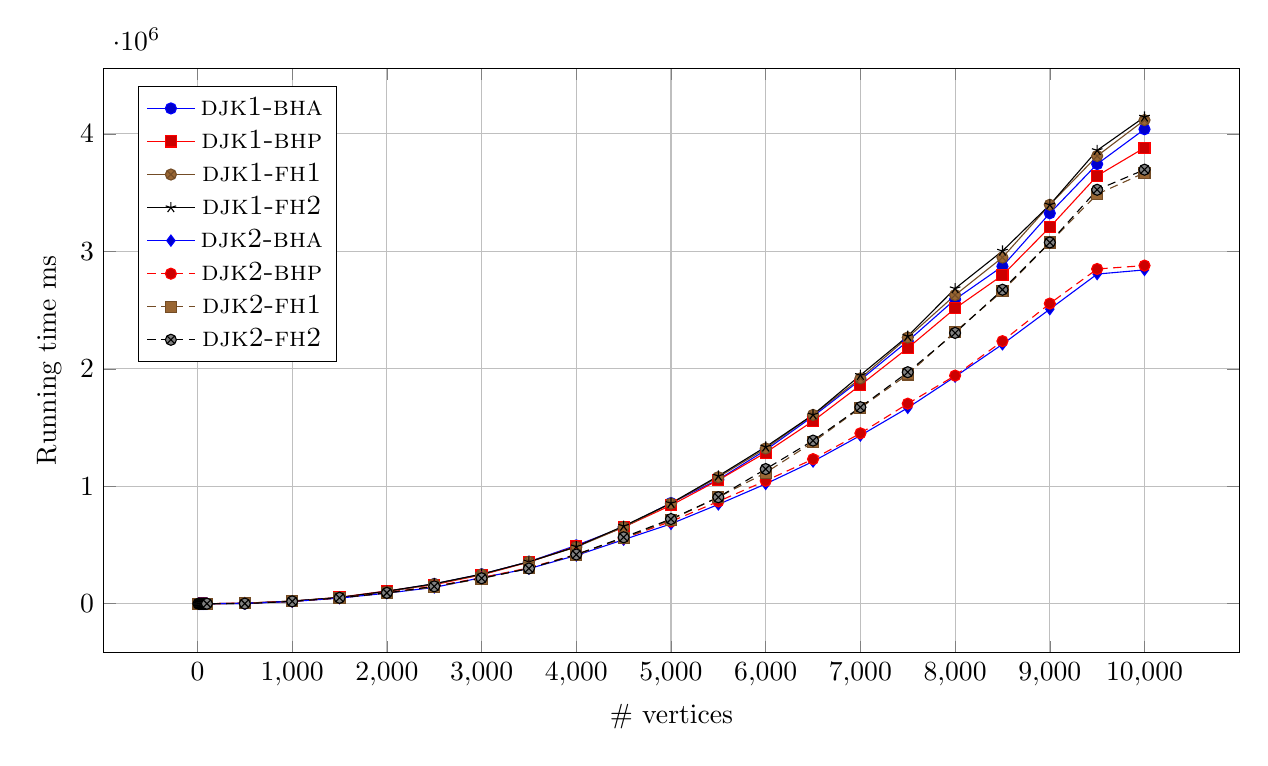
\begin{tikzpicture}
        \begin{axis}[
            xlabel = \# vertices,
            ylabel = Running time ms,
            height=9cm,
            width=16cm,
            grid=major,
            xtick={0,1000,2000,...,10000},
            scaled x ticks = false,
            legend pos=north west
    	]
    		
    		
    	\addplot coordinates {
(10,0)
(20,0)
(30,0)
(40,0)
(50,0)
(60,0)
(70,0)
(80,0)
(90,0)
(100,0)
(500,1111)
(1000,21111)
(1500,51111)
(2000,105555)
(2500,168888)
(3000,251111)
(3500,357777)
(4000,496666)
(4500,652222)
(5000,857777)
(5500,1056666)
(6000,1307777)
(6500,1595555)
(7000,1905555)
(7500,2235555)
(8000,2591111)
(8500,2872222)
(9000,3324444)
(9500,3743333)
(10000,4040000)

    	};
        
    	\addlegendentry{\textsc{djk1-bha}}

                \addplot coordinates {
(10,0)
(20,0)
(30,0)
(40,0)
(50,0)
(60,0)
(70,0)
(80,0)
(90,0)
(100,0)
(500,4444)
(1000,21111)
(1500,54444)
(2000,108888)
(2500,162222)
(3000,245555)
(3500,354444)
(4000,488888)
(4500,652222)
(5000,837777)
(5500,1052222)
(6000,1286666)
(6500,1555555)
(7000,1861111)
(7500,2176666)
(8000,2514444)
(8500,2796666)
(9000,3205555)
(9500,3643333)
(10000,3882222)

    	};
        
    	\addlegendentry{\textsc{djk1-bhp}}

        \addplot coordinates {
(10,0)
(20,0)
(30,0)
(40,0)
(50,0)
(60,0)
(70,0)
(80,0)
(90,0)
(100,0)
(500,4444)
(1000,22222)
(1500,52222)
(2000,103333)
(2500,167777)
(3000,248888)
(3500,357777)
(4000,482222)
(4500,652222)
(5000,853333)
(5500,1077777)
(6000,1322222)
(6500,1607777)
(7000,1918888)
(7500,2266666)
(8000,2627777)
(8500,2947777)
(9000,3396666)
(9500,3812222)
(10000,4117777)

    	};
        
    	\addlegendentry{\textsc{djk1-fh1}}

        \addplot coordinates {
(10,0)
(20,0)
(30,0)
(40,0)
(50,0)
(60,0)
(70,0)
(80,0)
(90,0)
(100,0)
(500,2222)
(1000,23333)
(1500,53333)
(2000,106666)
(2500,170000)
(3000,252222)
(3500,356666)
(4000,485555)
(4500,661111)
(5000,855555)
(5500,1087777)
(6000,1335555)
(6500,1608888)
(7000,1945555)
(7500,2277777)
(8000,2683333)
(8500,3003333)
(9000,3396666)
(9500,3860000)
(10000,4144444)

    	};
        
    	\addlegendentry{\textsc{djk1-fh2}}


        \addplot coordinates {
(10,0)
(20,0)
(30,0)
(40,0)
(50,0)
(60,0)
(70,0)
(80,0)
(90,0)
(100,0)
(500,4444)
(1000,18888)
(1500,47777)
(2000,90000)
(2500,138888)
(3000,222222)
(3500,298888)
(4000,411111)
(4500,545555)
(5000,680000)
(5500,845555)
(6000,1020000)
(6500,1211111)
(7000,1432222)
(7500,1667777)
(8000,1933333)
(8500,2208888)
(9000,2507777)
(9500,2806666)
(10000,2842222)
        };
        
    	\addlegendentry{\textsc{djk2-bha}}

        \addplot coordinates {
(10,0)
(20,0)
(30,0)
(40,0)
(50,0)
(60,0)
(70,0)
(80,0)
(90,0)
(100,0)
(500,5555)
(1000,21111)
(1500,48888)
(2000,95555)
(2500,147777)
(3000,222222)
(3500,305555)
(4000,420000)
(4500,556666)
(5000,700000)
(5500,871111)
(6000,1046666)
(6500,1231111)
(7000,1451111)
(7500,1703333)
(8000,1942222)
(8500,2235555)
(9000,2555555)
(9500,2850000)
(10000,2878888)
        };
        
        \addlegendentry{\textsc{djk2-bhp}}

        \addplot coordinates {
(10,0)
(20,0)
(30,0)
(40,0)
(50,0)
(60,0)
(70,0)
(80,0)
(90,0)
(100,0)
(500,3333)
(1000,20000)
(1500,50000)
(2000,90000)
(2500,143333)
(3000,214444)
(3500,302222)
(4000,415555)
(4500,557777)
(5000,714444)
(5500,906666)
(6000,1115555)
(6500,1375555)
(7000,1667777)
(7500,1952222)
(8000,2315555)
(8500,2661111)
(9000,3075555)
(9500,3486666)
(10000,3668888)
        };
        
        \addlegendentry{\textsc{djk2-fh1}}
        
        \addplot coordinates {
(10,0)
(20,0)
(30,0)
(40,0)
(50,0)
(60,0)
(70,0)
(80,0)
(90,0)
(100,0)
(500,1111)
(1000,20000)
(1500,50000)
(2000,92222)
(2500,147777)
(3000,216666)
(3500,300000)
(4000,418888)
(4500,565555)
(5000,721111)
(5500,906666)
(6000,1146666)
(6500,1388888)
(7000,1673333)
(7500,1971111)
(8000,2305555)
(8500,2673333)
(9000,3075555)
(9500,3524444)
(10000,3695555)
        };
        
        \addlegendentry{\textsc{djk2-fh2}}

        \end{axis}

    \end{tikzpicture}
    \captionof{figure}{Average time of running \textsc{Dijkstra1} and \textsc{Dijkstra2} on 80 \% connected graph}
    \label{fig:sample_figure}
\end{minipage}

\begin{minipage}[c]{\textwidth}
\centering
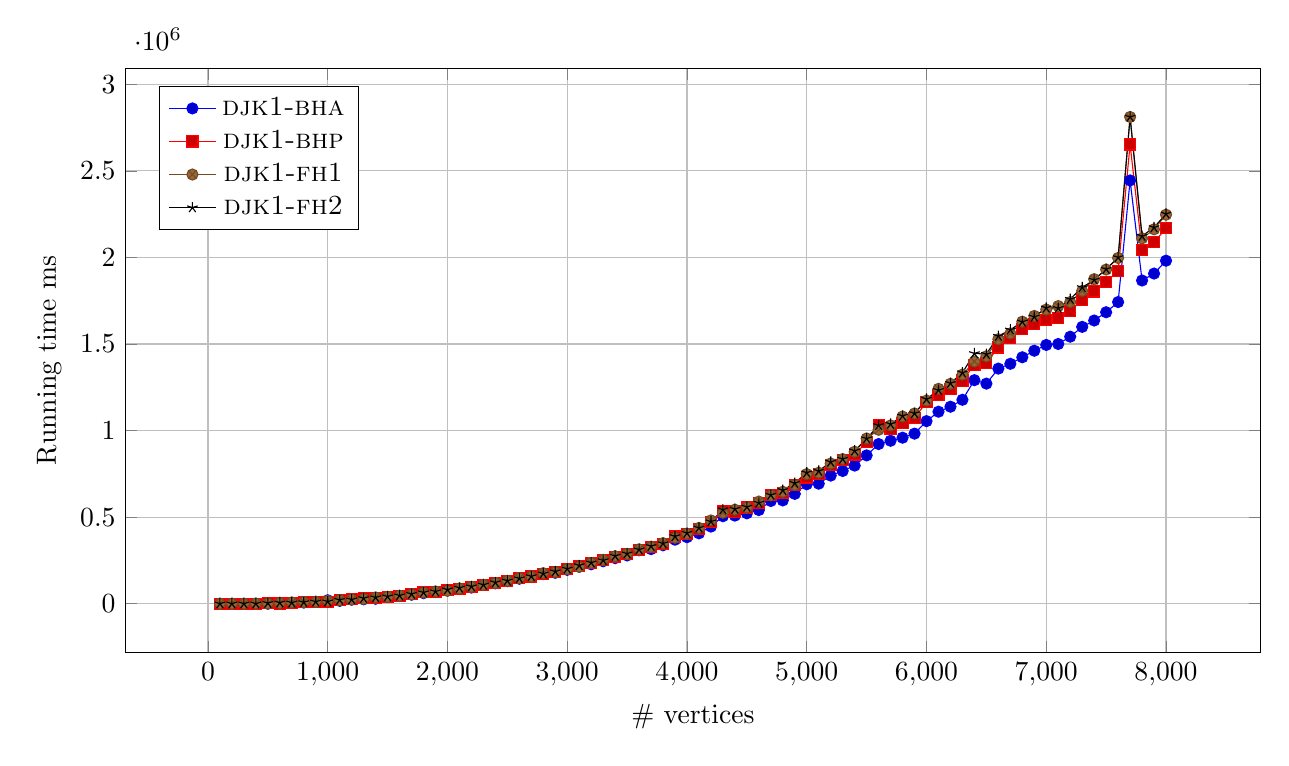
\begin{tikzpicture}
        \begin{axis}[
            xlabel = \# vertices,
            ylabel = Running time ms,
            height=9cm,
            width=16cm,
            grid=major,
            legend pos=north west
    	]
    		
    	\addplot coordinates {
(100,0)
(200,0)
(300,0)
(400,0)
(500,0)
(600,5555)
(700,4444)
(800,6666)
(900,11111)
(1000,20000)
(1100,16666)
(1200,23333)
(1300,25555)
(1400,28888)
(1500,38888)
(1600,44444)
(1700,52222)
(1800,61111)
(1900,67777)
(2000,77777)
(2100,84444)
(2200,93333)
(2300,108888)
(2400,117777)
(2500,130000)
(2600,144444)
(2700,154444)
(2800,171111)
(2900,178888)
(3000,195555)
(3100,213333)
(3200,227777)
(3300,245555)
(3400,263333)
(3500,278888)
(3600,308888)
(3700,315555)
(3800,337777)
(3900,370000)
(4000,384444)
(4100,406666)
(4200,445555)
(4300,505555)
(4400,508888)
(4500,522222)
(4600,541111)
(4700,593333)
(4800,596666)
(4900,634444)
(5000,690000)
(5100,693333)
(5200,740000)
(5300,766666)
(5400,797777)
(5500,856666)
(5600,922222)
(5700,941111)
(5800,958888)
(5900,982222)
(6000,1054444)
(6100,1108888)
(6200,1137777)
(6300,1177777)
(6400,1291111)
(6500,1271111)
(6600,1357777)
(6700,1385555)
(6800,1423333)
(6900,1461111)
(7000,1494444)
(7100,1500000)
(7200,1542222)
(7300,1598888)
(7400,1635555)
(7500,1683333)
(7600,1742222)
(7700,2444444)
(7800,1866666)
(7900,1906666)
(8000,1981111)
    	};
        
    	\addlegendentry{\textsc{djk1-bha}}

                \addplot coordinates {
(100,0)
(200,0)
(300,0)
(400,0)
(500,4444)
(600,1111)
(700,5555)
(800,7777)
(900,11111)
(1000,12222)
(1100,20000)
(1200,25555)
(1300,32222)
(1400,34444)
(1500,40000)
(1600,46666)
(1700,54444)
(1800,66666)
(1900,70000)
(2000,80000)
(2100,86666)
(2200,96666)
(2300,106666)
(2400,117777)
(2500,131111)
(2600,147777)
(2700,157777)
(2800,172222)
(2900,184444)
(3000,200000)
(3100,217777)
(3200,235555)
(3300,252222)
(3400,270000)
(3500,285555)
(3600,308888)
(3700,327777)
(3800,344444)
(3900,387777)
(4000,404444)
(4100,433333)
(4200,470000)
(4300,533333)
(4400,532222)
(4500,555555)
(4600,580000)
(4700,628888)
(4800,638888)
(4900,685555)
(5000,728888)
(5100,747777)
(5200,803333)
(5300,828888)
(5400,862222)
(5500,933333)
(5600,1033333)
(5700,1008888)
(5800,1044444)
(5900,1073333)
(6000,1163333)
(6100,1205555)
(6200,1240000)
(6300,1288888)
(6400,1380000)
(6500,1391111)
(6600,1480000)
(6700,1534444)
(6800,1585555)
(6900,1616666)
(7000,1636666)
(7100,1648888)
(7200,1690000)
(7300,1756666)
(7400,1803333)
(7500,1857777)
(7600,1922222)
(7700,2652222)
(7800,2041111)
(7900,2086666)
(8000,2167777)
    	};
        
    	\addlegendentry{\textsc{djk1-bhp}}

        \addplot coordinates {
(100,0)
(200,0)
(300,0)
(400,1111)
(500,1111)
(600,3333)
(700,7777)
(800,10000)
(900,11111)
(1000,16666)
(1100,21111)
(1200,24444)
(1300,27777)
(1400,36666)
(1500,40000)
(1600,46666)
(1700,53333)
(1800,64444)
(1900,71111)
(2000,74444)
(2100,87777)
(2200,97777)
(2300,108888)
(2400,120000)
(2500,132222)
(2600,147777)
(2700,156666)
(2800,176666)
(2900,183333)
(3000,200000)
(3100,213333)
(3200,235555)
(3300,253333)
(3400,274444)
(3500,287777)
(3600,314444)
(3700,327777)
(3800,350000)
(3900,381111)
(4000,404444)
(4100,437777)
(4200,481111)
(4300,525555)
(4400,543333)
(4500,555555)
(4600,590000)
(4700,625555)
(4800,646666)
(4900,685555)
(5000,748888)
(5100,756666)
(5200,810000)
(5300,835555)
(5400,877777)
(5500,954444)
(5600,1004444)
(5700,1030000)
(5800,1081111)
(5900,1098888)
(6000,1173333)
(6100,1241111)
(6200,1270000)
(6300,1323333)
(6400,1398888)
(6500,1428888)
(6600,1527777)
(6700,1561111)
(6800,1628888)
(6900,1662222)
(7000,1698888)
(7100,1718888)
(7200,1742222)
(7300,1806666)
(7400,1874444)
(7500,1930000)
(7600,1996666)
(7700,2811111)
(7800,2110000)
(7900,2162222)
(8000,2246666)
    	};
        
    	\addlegendentry{\textsc{djk1-fh1}}

        \addplot coordinates {
(100,0)
(200,0)
(300,0)
(400,0)
(500,3333)
(600,5555)
(700,5555)
(800,7777)
(900,11111)
(1000,12222)
(1100,21111)
(1200,23333)
(1300,31111)
(1400,35555)
(1500,41111)
(1600,46666)
(1700,55555)
(1800,64444)
(1900,70000)
(2000,81111)
(2100,91111)
(2200,98888)
(2300,108888)
(2400,122222)
(2500,132222)
(2600,145555)
(2700,157777)
(2800,173333)
(2900,185555)
(3000,201111)
(3100,221111)
(3200,236666)
(3300,250000)
(3400,275555)
(3500,288888)
(3600,312222)
(3700,332222)
(3800,347777)
(3900,388888)
(4000,407777)
(4100,437777)
(4200,474444)
(4300,543333)
(4400,546666)
(4500,558888)
(4600,582222)
(4700,627777)
(4800,655555)
(4900,696666)
(5000,756666)
(5100,766666)
(5200,818888)
(5300,835555)
(5400,883333)
(5500,953333)
(5600,1030000)
(5700,1037777)
(5800,1084444)
(5900,1098888)
(6000,1182222)
(6100,1233333)
(6200,1273333)
(6300,1334444)
(6400,1445555)
(6500,1441111)
(6600,1545555)
(6700,1582222)
(6800,1627777)
(6900,1656666)
(7000,1708888)
(7100,1706666)
(7200,1758888)
(7300,1826666)
(7400,1870000)
(7500,1932222)
(7600,2000000)
(7700,2811111)
(7800,2123333)
(7900,2173333)
(8000,2251111)
    	};
        
    	\addlegendentry{\textsc{djk1-fh2}}


        \addplot coordinates {
        };
        
    	\addlegendentry{\textsc{djk2-bha}}

        \addplot coordinates {
        };
        
        \addlegendentry{\textsc{djk2-bhp}}

        \addplot coordinates {
        };
        
        \addlegendentry{\textsc{djk2-fh1}}
        
        \addplot coordinates {
        };
        
        \addlegendentry{\textsc{djk2-fh2}}

        \end{axis}

    \end{tikzpicture}
    \captionof{figure}{Average time of running \textsc{Dijkstra1} and \textsc{Dijkstra2} on 70 \% connected graph}
    \label{fig:sample_figure}
\end{minipage}

\begin{minipage}[c]{\textwidth}
\centering
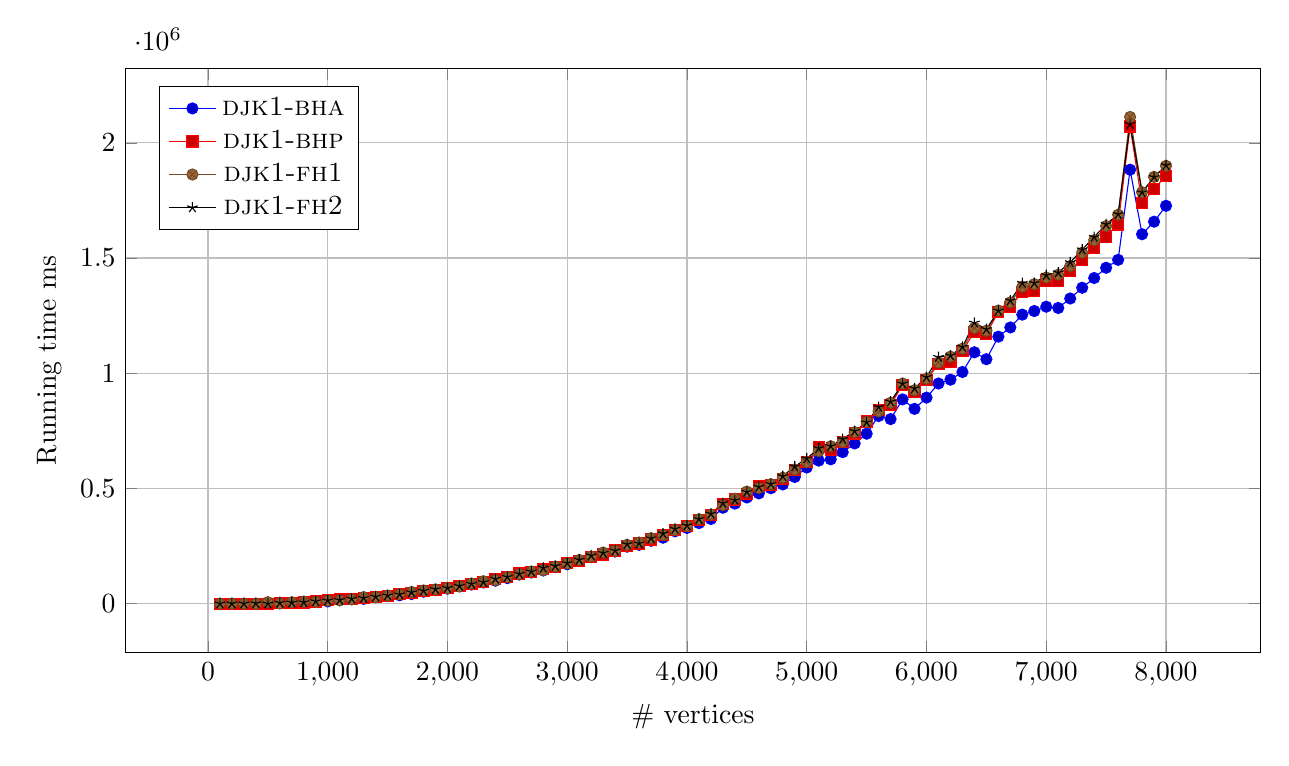
\begin{tikzpicture}
        \begin{axis}[
            xlabel = \# vertices,
            ylabel = Running time ms,
            height=9cm,
            width=16cm,
            grid=major,
            legend pos=north west
    	]
    		
    	\addplot coordinates {
(100,0)
(200,0)
(300,0)
(400,0)
(500,0)
(600,4444)
(700,3333)
(800,8888)
(900,8888)
(1000,10000)
(1100,17777)
(1200,20000)
(1300,21111)
(1400,28888)
(1500,33333)
(1600,36666)
(1700,42222)
(1800,52222)
(1900,60000)
(2000,65555)
(2100,76666)
(2200,83333)
(2300,92222)
(2400,100000)
(2500,111111)
(2600,126666)
(2700,135555)
(2800,144444)
(2900,158888)
(3000,171111)
(3100,186666)
(3200,202222)
(3300,212222)
(3400,226666)
(3500,247777)
(3600,255555)
(3700,273333)
(3800,286666)
(3900,314444)
(4000,328888)
(4100,350000)
(4200,367777)
(4300,416666)
(4400,434444)
(4500,461111)
(4600,478888)
(4700,501111)
(4800,517777)
(4900,550000)
(5000,591111)
(5100,621111)
(5200,626666)
(5300,657777)
(5400,695555)
(5500,737777)
(5600,814444)
(5700,801111)
(5800,886666)
(5900,845555)
(6000,894444)
(6100,955555)
(6200,972222)
(6300,1005555)
(6400,1091111)
(6500,1061111)
(6600,1158888)
(6700,1198888)
(6800,1254444)
(6900,1270000)
(7000,1288888)
(7100,1283333)
(7200,1324444)
(7300,1371111)
(7400,1413333)
(7500,1457777)
(7600,1492222)
(7700,1883333)
(7800,1603333)
(7900,1657777)
(8000,1726666)
    	};
        
    	\addlegendentry{\textsc{djk1-bha}}

                \addplot coordinates {
(100,0)
(200,0)
(300,0)
(400,0)
(500,0)
(600,3333)
(700,4444)
(800,5555)
(900,10000)
(1000,14444)
(1100,18888)
(1200,21111)
(1300,23333)
(1400,30000)
(1500,32222)
(1600,42222)
(1700,47777)
(1800,56666)
(1900,61111)
(2000,70000)
(2100,77777)
(2200,86666)
(2300,93333)
(2400,107777)
(2500,115555)
(2600,131111)
(2700,136666)
(2800,150000)
(2900,161111)
(3000,175555)
(3100,185555)
(3200,204444)
(3300,213333)
(3400,231111)
(3500,252222)
(3600,261111)
(3700,278888)
(3800,300000)
(3900,318888)
(4000,335555)
(4100,363333)
(4200,385555)
(4300,434444)
(4400,452222)
(4500,476666)
(4600,510000)
(4700,516666)
(4800,540000)
(4900,578888)
(5000,613333)
(5100,678888)
(5200,666666)
(5300,700000)
(5400,738888)
(5500,791111)
(5600,838888)
(5700,862222)
(5800,950000)
(5900,918888)
(6000,972222)
(6100,1040000)
(6200,1048888)
(6300,1096666)
(6400,1180000)
(6500,1170000)
(6600,1266666)
(6700,1288888)
(6800,1351111)
(6900,1357777)
(7000,1402222)
(7100,1401111)
(7200,1445555)
(7300,1492222)
(7400,1544444)
(7500,1593333)
(7600,1645555)
(7700,2071111)
(7800,1737777)
(7900,1801111)
(8000,1855555)
    	};
        
    	\addlegendentry{\textsc{djk1-bhp}}

        \addplot coordinates {
(100,0)
(200,0)
(300,0)
(400,0)
(500,6666)
(600,1111)
(700,6666)
(800,8888)
(900,8888)
(1000,13333)
(1100,14444)
(1200,18888)
(1300,28888)
(1400,28888)
(1500,35555)
(1600,41111)
(1700,51111)
(1800,57777)
(1900,62222)
(2000,67777)
(2100,74444)
(2200,87777)
(2300,97777)
(2400,102222)
(2500,115555)
(2600,128888)
(2700,140000)
(2800,145555)
(2900,161111)
(3000,174444)
(3100,190000)
(3200,204444)
(3300,222222)
(3400,230000)
(3500,255555)
(3600,265555)
(3700,284444)
(3800,297777)
(3900,320000)
(4000,336666)
(4100,366666)
(4200,386666)
(4300,427777)
(4400,455555)
(4500,486666)
(4600,502222)
(4700,518888)
(4800,546666)
(4900,582222)
(5000,614444)
(5100,662222)
(5200,683333)
(5300,702222)
(5400,744444)
(5500,788888)
(5600,834444)
(5700,872222)
(5800,955555)
(5900,926666)
(6000,976666)
(6100,1046666)
(6200,1072222)
(6300,1106666)
(6400,1196666)
(6500,1184444)
(6600,1272222)
(6700,1307777)
(6800,1375555)
(6900,1386666)
(7000,1415555)
(7100,1427777)
(7200,1465555)
(7300,1523333)
(7400,1577777)
(7500,1638888)
(7600,1687777)
(7700,2112222)
(7800,1785555)
(7900,1852222)
(8000,1900000)
    	};
        
    	\addlegendentry{\textsc{djk1-fh1}}

        \addplot coordinates {
(100,0)
(200,0)
(300,0)
(400,1111)
(500,0)
(600,3333)
(700,4444)
(800,5555)
(900,10000)
(1000,13333)
(1100,15555)
(1200,21111)
(1300,24444)
(1400,30000)
(1500,35555)
(1600,40000)
(1700,48888)
(1800,55555)
(1900,62222)
(2000,67777)
(2100,76666)
(2200,85555)
(2300,93333)
(2400,107777)
(2500,115555)
(2600,128888)
(2700,138888)
(2800,155555)
(2900,163333)
(3000,175555)
(3100,190000)
(3200,208888)
(3300,220000)
(3400,230000)
(3500,257777)
(3600,261111)
(3700,283333)
(3800,304444)
(3900,324444)
(4000,338888)
(4100,366666)
(4200,390000)
(4300,436666)
(4400,448888)
(4500,484444)
(4600,506666)
(4700,518888)
(4800,553333)
(4900,595555)
(5000,630000)
(5100,674444)
(5200,683333)
(5300,714444)
(5400,748888)
(5500,786666)
(5600,853333)
(5700,876666)
(5800,954444)
(5900,934444)
(6000,983333)
(6100,1070000)
(6200,1076666)
(6300,1114444)
(6400,1218888)
(6500,1191111)
(6600,1271111)
(6700,1315555)
(6800,1391111)
(6900,1391111)
(7000,1425555)
(7100,1436666)
(7200,1481111)
(7300,1536666)
(7400,1591111)
(7500,1646666)
(7600,1690000)
(7700,2081111)
(7800,1784444)
(7900,1851111)
(8000,1902222)
    	};
        
    	\addlegendentry{\textsc{djk1-fh2}}


        \addplot coordinates {
        };
        
    	\addlegendentry{\textsc{djk2-bha}}

        \addplot coordinates {
        };
        
        \addlegendentry{\textsc{djk2-bhp}}

        \addplot coordinates {
        };
        
        \addlegendentry{\textsc{djk2-fh1}}
        
        \addplot coordinates {
        };
        
        \addlegendentry{\textsc{djk2-fh2}}

        \end{axis}

    \end{tikzpicture}
    \captionof{figure}{Average time of running \textsc{Dijkstra1} and \textsc{Dijkstra2} on 60 \% connected graph}
    \label{fig:sample_figure}
\end{minipage}

\begin{minipage}[c]{\textwidth}
\centering
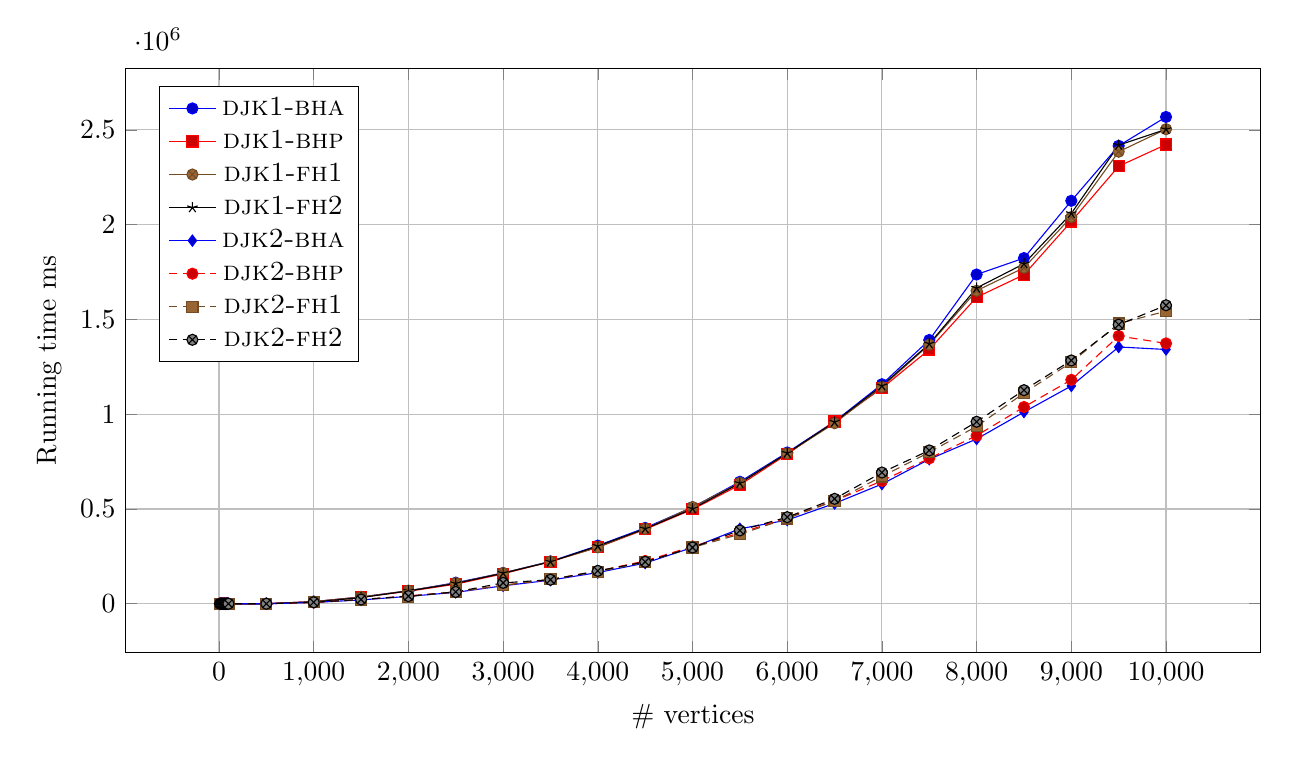
\begin{tikzpicture}
        \begin{axis}[
            xlabel = \# vertices,
            ylabel = Running time ms,
            height=9cm,
            width=16cm,
            grid=major,
            xtick={0,1000,2000,...,10000},
            scaled x ticks = false,
            legend pos=north west
    	]
    		
    		
    	\addplot coordinates {
(10,0)
(20,0)
(30,0)
(40,0)
(50,0)
(60,0)
(70,0)
(80,0)
(90,0)
(100,0)
(500,0)
(1000,11111)
(1500,35555)
(2000,67777)
(2500,111111)
(3000,162222)
(3500,223333)
(4000,306666)
(4500,400000)
(5000,508888)
(5500,643333)
(6000,797777)
(6500,961111)
(7000,1157777)
(7500,1391111)
(8000,1736666)
(8500,1823333)
(9000,2125555)
(9500,2415555)
(10000,2567777)

    	};
        
    	\addlegendentry{\textsc{djk1-bha}}

                \addplot coordinates {
(10,0)
(20,0)
(30,0)
(40,0)
(50,0)
(60,0)
(70,0)
(80,0)
(90,0)
(100,0)
(500,0)
(1000,11111)
(1500,34444)
(2000,65555)
(2500,103333)
(3000,157777)
(3500,222222)
(4000,297777)
(4500,392222)
(5000,497777)
(5500,626666)
(6000,788888)
(6500,961111)
(7000,1136666)
(7500,1341111)
(8000,1616666)
(8500,1735555)
(9000,2016666)
(9500,2307777)
(10000,2422222)

    	};
        
    	\addlegendentry{\textsc{djk1-bhp}}

        \addplot coordinates {
(10,0)
(20,0)
(30,0)
(40,0)
(50,0)
(60,0)
(70,0)
(80,0)
(90,0)
(100,0)
(500,0)
(1000,11111)
(1500,35555)
(2000,68888)
(2500,108888)
(3000,162222)
(3500,222222)
(4000,297777)
(4500,395555)
(5000,510000)
(5500,637777)
(6000,793333)
(6500,952222)
(7000,1143333)
(7500,1366666)
(8000,1651111)
(8500,1772222)
(9000,2040000)
(9500,2384444)
(10000,2503333)

    	};
        
    	\addlegendentry{\textsc{djk1-fh1}}

        \addplot coordinates {
(10,0)
(20,0)
(30,0)
(40,0)
(50,0)
(60,0)
(70,0)
(80,0)
(90,0)
(100,0)
(500,0)
(1000,8888)
(1500,32222)
(2000,67777)
(2500,106666)
(3000,161111)
(3500,221111)
(4000,304444)
(4500,395555)
(5000,501111)
(5500,635555)
(6000,794444)
(6500,958888)
(7000,1150000)
(7500,1371111)
(8000,1665555)
(8500,1793333)
(9000,2058888)
(9500,2418888)
(10000,2502222)

    	};
        
    	\addlegendentry{\textsc{djk1-fh2}}


        \addplot coordinates {
(10,0)
(20,0)
(30,0)
(40,0)
(50,0)
(60,0)
(70,0)
(80,0)
(90,0)
(100,0)
(500,0)
(1000,6666)
(1500,20000)
(2000,38888)
(2500,60000)
(3000,94444)
(3500,124444)
(4000,164444)
(4500,214444)
(5000,296666)
(5500,395555)
(6000,441111)
(6500,528888)
(7000,631111)
(7500,762222)
(8000,868888)
(8500,1011111)
(9000,1148888)
(9500,1354444)
(10000,1341111)
        };
        
    	\addlegendentry{\textsc{djk2-bha}}

        \addplot coordinates {
(10,0)
(20,0)
(30,0)
(40,0)
(50,0)
(60,0)
(70,0)
(80,0)
(90,0)
(100,0)
(500,0)
(1000,6666)
(1500,22222)
(2000,41111)
(2500,62222)
(3000,97777)
(3500,127777)
(4000,172222)
(4500,225555)
(5000,302222)
(5500,373333)
(6000,453333)
(6500,543333)
(7000,647777)
(7500,766666)
(8000,886666)
(8500,1037777)
(9000,1181111)
(9500,1412222)
(10000,1373333)
        };
        
        \addlegendentry{\textsc{djk2-bhp}}

        \addplot coordinates {
(10,0)
(20,0)
(30,0)
(40,0)
(50,0)
(60,0)
(70,0)
(80,0)
(90,0)
(100,0)
(500,0)
(1000,7777)
(1500,22222)
(2000,37777)
(2500,63333)
(3000,96666)
(3500,128888)
(4000,168888)
(4500,218888)
(5000,296666)
(5500,366666)
(6000,450000)
(6500,542222)
(7000,671111)
(7500,798888)
(8000,935555)
(8500,1111111)
(9000,1273333)
(9500,1477777)
(10000,1543333)
        };
        
        \addlegendentry{\textsc{djk2-fh1}}
        
        \addplot coordinates {
(10,0)
(20,0)
(30,0)
(40,0)
(50,0)
(60,0)
(70,0)
(80,0)
(90,0)
(100,0)
(500,0)
(1000,7777)
(1500,22222)
(2000,40000)
(2500,62222)
(3000,110000)
(3500,126666)
(4000,173333)
(4500,221111)
(5000,296666)
(5500,386666)
(6000,456666)
(6500,553333)
(7000,692222)
(7500,808888)
(8000,960000)
(8500,1126666)
(9000,1283333)
(9500,1472222)
(10000,1574444)
        };
        
        \addlegendentry{\textsc{djk2-fh2}}

        \end{axis}

    \end{tikzpicture}
    \captionof{figure}{Average time of running \textsc{Dijkstra1} and \textsc{Dijkstra2} on 50 \% connected graph}
    \label{fig:sample_figure}
\end{minipage}

\begin{minipage}[c]{\textwidth}
\centering
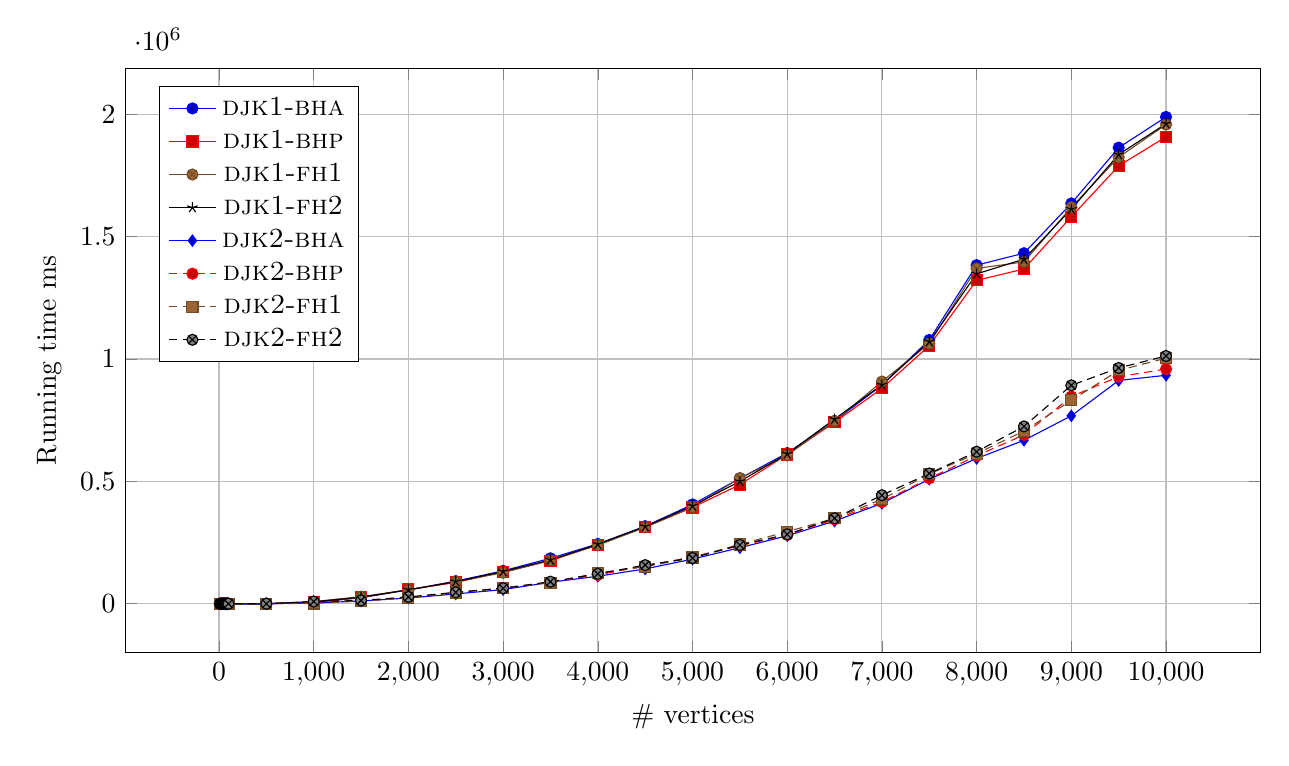
\begin{tikzpicture}
        \begin{axis}[
            xlabel = \# vertices,
            ylabel = Running time ms,
            height=9cm,
            width=16cm,
            grid=major,
            xtick={0,1000,2000,...,10000},
            scaled x ticks = false,
            legend pos=north west
    	]
    		
    		
    	\addplot coordinates {
(10,0)
(20,0)
(30,0)
(40,0)
(50,0)
(60,0)
(70,0)
(80,0)
(90,0)
(100,0)
(500,0)
(1000,5555)
(1500,24444)
(2000,56666)
(2500,92222)
(3000,134444)
(3500,185555)
(4000,244444)
(4500,316666)
(5000,405555)
(5500,512222)
(6000,615555)
(6500,746666)
(7000,893333)
(7500,1077777)
(8000,1383333)
(8500,1432222)
(9000,1635555)
(9500,1863333)
(10000,1988888)

    	};
        
    	\addlegendentry{\textsc{djk1-bha}}

                \addplot coordinates {
(10,0)
(20,0)
(30,0)
(40,0)
(50,0)
(60,0)
(70,0)
(80,0)
(90,0)
(100,0)
(500,0)
(1000,5555)
(1500,25555)
(2000,57777)
(2500,86666)
(3000,130000)
(3500,175555)
(4000,241111)
(4500,313333)
(5000,393333)
(5500,486666)
(6000,610000)
(6500,741111)
(7000,880000)
(7500,1054444)
(8000,1321111)
(8500,1367777)
(9000,1581111)
(9500,1788888)
(10000,1907777)

    	};
        
    	\addlegendentry{\textsc{djk1-bhp}}

        \addplot coordinates {
(10,0)
(20,0)
(30,0)
(40,0)
(50,0)
(60,0)
(70,0)
(80,0)
(90,0)
(100,0)
(500,0)
(1000,8888)
(1500,28888)
(2000,56666)
(2500,90000)
(3000,126666)
(3500,177777)
(4000,238888)
(4500,312222)
(5000,394444)
(5500,513333)
(6000,606666)
(6500,746666)
(7000,907777)
(7500,1063333)
(8000,1370000)
(8500,1396666)
(9000,1620000)
(9500,1824444)
(10000,1957777)

    	};
        
    	\addlegendentry{\textsc{djk1-fh1}}

        \addplot coordinates {
(10,0)
(20,0)
(30,0)
(40,0)
(50,0)
(60,0)
(70,0)
(80,0)
(90,0)
(100,0)
(500,0)
(1000,7777)
(1500,26666)
(2000,56666)
(2500,90000)
(3000,132222)
(3500,178888)
(4000,243333)
(4500,315555)
(5000,400000)
(5500,500000)
(6000,612222)
(6500,754444)
(7000,894444)
(7500,1071111)
(8000,1347777)
(8500,1407777)
(9000,1612222)
(9500,1835555)
(10000,1961111)

    	};
        
    	\addlegendentry{\textsc{djk1-fh2}}


        \addplot coordinates {
(10,0)
(20,0)
(30,0)
(40,0)
(50,0)
(60,0)
(70,0)
(80,0)
(90,0)
(100,0)
(500,0)
(1000,3333)
(1500,11111)
(2000,23333)
(2500,40000)
(3000,57777)
(3500,87777)
(4000,112222)
(4500,142222)
(5000,182222)
(5500,228888)
(6000,277777)
(6500,337777)
(7000,410000)
(7500,508888)
(8000,593333)
(8500,667777)
(9000,767777)
(9500,912222)
(10000,933333)
        };
        
    	\addlegendentry{\textsc{djk2-bha}}

        \addplot coordinates {
(10,0)
(20,0)
(30,0)
(40,0)
(50,0)
(60,0)
(70,0)
(80,0)
(90,0)
(100,0)
(500,0)
(1000,6666)
(1500,11111)
(2000,24444)
(2500,45555)
(3000,63333)
(3500,87777)
(4000,117777)
(4500,154444)
(5000,191111)
(5500,236666)
(6000,281111)
(6500,344444)
(7000,415555)
(7500,512222)
(8000,604444)
(8500,690000)
(9000,846666)
(9500,927777)
(10000,958888)
        };
        
        \addlegendentry{\textsc{djk2-bhp}}

        \addplot coordinates {
(10,0)
(20,0)
(30,0)
(40,0)
(50,0)
(60,0)
(70,0)
(80,0)
(90,0)
(100,0)
(500,0)
(1000,1111)
(1500,11111)
(2000,24444)
(2500,45555)
(3000,64444)
(3500,85555)
(4000,125555)
(4500,151111)
(5000,188888)
(5500,242222)
(6000,294444)
(6500,348888)
(7000,426666)
(7500,530000)
(8000,613333)
(8500,705555)
(9000,831111)
(9500,953333)
(10000,1003333)
        };
        
        \addlegendentry{\textsc{djk2-fh1}}
        
        \addplot coordinates {
(10,0)
(20,0)
(30,0)
(40,0)
(50,0)
(60,0)
(70,0)
(80,0)
(90,0)
(100,0)
(500,0)
(1000,8888)
(1500,13333)
(2000,27777)
(2500,46666)
(3000,63333)
(3500,90000)
(4000,122222)
(4500,157777)
(5000,186666)
(5500,240000)
(6000,283333)
(6500,348888)
(7000,443333)
(7500,532222)
(8000,621111)
(8500,724444)
(9000,892222)
(9500,963333)
(10000,1012222)
        };
        
        \addlegendentry{\textsc{djk2-fh2}}

        \end{axis}

    \end{tikzpicture}
    \captionof{figure}{Average time of running \textsc{Dijkstra1} and \textsc{Dijkstra2} on 40 \% connected graph}
    \label{fig:sample_figure}
\end{minipage}

\begin{minipage}[c]{\textwidth}
\centering
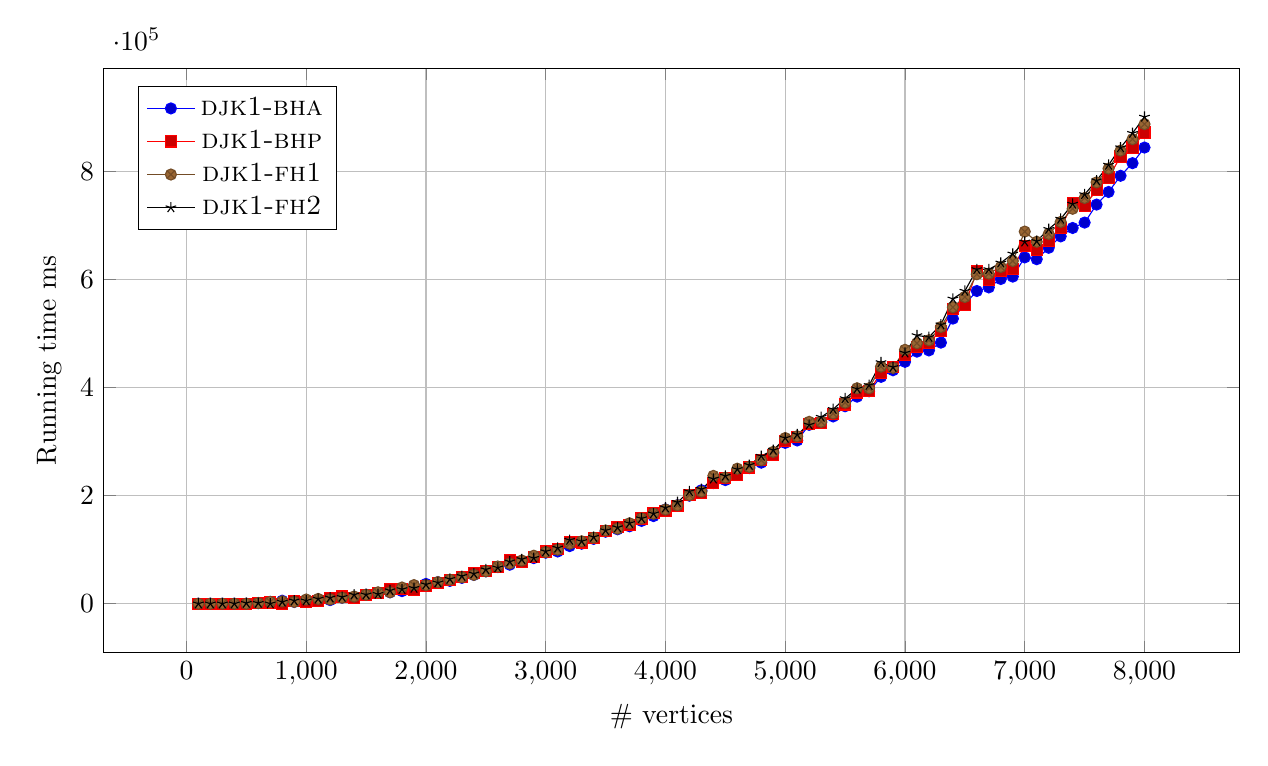
\begin{tikzpicture}
        \begin{axis}[
            xlabel = \# vertices,
            ylabel = Running time ms,
            height=9cm,
            width=16cm,
            grid=major,
            legend pos=north west
    	]
    		
    	\addplot coordinates {
(100,0)
(200,0)
(300,0)
(400,0)
(500,0)
(600,1111)
(700,3333)
(800,5555)
(900,3333)
(1000,6666)
(1100,5555)
(1200,6666)
(1300,11111)
(1400,12222)
(1500,16666)
(1600,20000)
(1700,21111)
(1800,23333)
(1900,33333)
(2000,36666)
(2100,40000)
(2200,42222)
(2300,47777)
(2400,53333)
(2500,60000)
(2600,67777)
(2700,72222)
(2800,78888)
(2900,84444)
(3000,94444)
(3100,96666)
(3200,106666)
(3300,111111)
(3400,120000)
(3500,133333)
(3600,137777)
(3700,143333)
(3800,153333)
(3900,162222)
(4000,174444)
(4100,182222)
(4200,200000)
(4300,210000)
(4400,223333)
(4500,228888)
(4600,244444)
(4700,251111)
(4800,261111)
(4900,278888)
(5000,297777)
(5100,302222)
(5200,331111)
(5300,335555)
(5400,346666)
(5500,365555)
(5600,383333)
(5700,393333)
(5800,420000)
(5900,432222)
(6000,447777)
(6100,466666)
(6200,468888)
(6300,483333)
(6400,527777)
(6500,554444)
(6600,578888)
(6700,585555)
(6800,601111)
(6900,605555)
(7000,641111)
(7100,637777)
(7200,658888)
(7300,680000)
(7400,695555)
(7500,705555)
(7600,738888)
(7700,762222)
(7800,792222)
(7900,815555)
(8000,844444)
    	};
        
    	\addlegendentry{\textsc{djk1-bha}}

                \addplot coordinates {
(100,0)
(200,0)
(300,0)
(400,0)
(500,0)
(600,1111)
(700,2222)
(800,0)
(900,4444)
(1000,3333)
(1100,5555)
(1200,10000)
(1300,13333)
(1400,11111)
(1500,16666)
(1600,20000)
(1700,26666)
(1800,26666)
(1900,25555)
(2000,32222)
(2100,38888)
(2200,43333)
(2300,50000)
(2400,56666)
(2500,61111)
(2600,67777)
(2700,81111)
(2800,76666)
(2900,86666)
(3000,96666)
(3100,101111)
(3200,114444)
(3300,113333)
(3400,122222)
(3500,134444)
(3600,142222)
(3700,145555)
(3800,157777)
(3900,167777)
(4000,171111)
(4100,181111)
(4200,201111)
(4300,205555)
(4400,223333)
(4500,233333)
(4600,237777)
(4700,252222)
(4800,265555)
(4900,275555)
(5000,301111)
(5100,308888)
(5200,333333)
(5300,334444)
(5400,351111)
(5500,368888)
(5600,391111)
(5700,393333)
(5800,427777)
(5900,437777)
(6000,461111)
(6100,475555)
(6200,483333)
(6300,505555)
(6400,545555)
(6500,552222)
(6600,615555)
(6700,598888)
(6800,615555)
(6900,620000)
(7000,662222)
(7100,655555)
(7200,672222)
(7300,695555)
(7400,741111)
(7500,736666)
(7600,765555)
(7700,788888)
(7800,827777)
(7900,844444)
(8000,872222)
    	};
        
    	\addlegendentry{\textsc{djk1-bhp}}

        \addplot coordinates {
(100,0)
(200,0)
(300,0)
(400,0)
(500,0)
(600,1111)
(700,3333)
(800,4444)
(900,3333)
(1000,7777)
(1100,8888)
(1200,7777)
(1300,11111)
(1400,13333)
(1500,16666)
(1600,21111)
(1700,21111)
(1800,30000)
(1900,34444)
(2000,34444)
(2100,40000)
(2200,44444)
(2300,48888)
(2400,53333)
(2500,60000)
(2600,68888)
(2700,74444)
(2800,80000)
(2900,88888)
(3000,95555)
(3100,100000)
(3200,111111)
(3300,115555)
(3400,122222)
(3500,135555)
(3600,138888)
(3700,148888)
(3800,157777)
(3900,166666)
(4000,174444)
(4100,182222)
(4200,201111)
(4300,207777)
(4400,236666)
(4500,233333)
(4600,250000)
(4700,253333)
(4800,265555)
(4900,281111)
(5000,306666)
(5100,310000)
(5200,336666)
(5300,336666)
(5400,352222)
(5500,372222)
(5600,398888)
(5700,398888)
(5800,438888)
(5900,436666)
(6000,470000)
(6100,482222)
(6200,487777)
(6300,512222)
(6400,548888)
(6500,567777)
(6600,610000)
(6700,611111)
(6800,623333)
(6900,634444)
(7000,688888)
(7100,670000)
(7200,684444)
(7300,706666)
(7400,731111)
(7500,751111)
(7600,780000)
(7700,805555)
(7800,838888)
(7900,860000)
(8000,887777)
    	};
        
    	\addlegendentry{\textsc{djk1-fh1}}

        \addplot coordinates {
(100,0)
(200,0)
(300,0)
(400,0)
(500,1111)
(600,1111)
(700,0)
(800,3333)
(900,5555)
(1000,5555)
(1100,8888)
(1200,11111)
(1300,12222)
(1400,16666)
(1500,16666)
(1600,17777)
(1700,24444)
(1800,26666)
(1900,28888)
(2000,35555)
(2100,38888)
(2200,45555)
(2300,51111)
(2400,55555)
(2500,63333)
(2600,66666)
(2700,77777)
(2800,82222)
(2900,84444)
(3000,96666)
(3100,103333)
(3200,117777)
(3300,115555)
(3400,123333)
(3500,135555)
(3600,141111)
(3700,148888)
(3800,157777)
(3900,166666)
(4000,177777)
(4100,187777)
(4200,207777)
(4300,212222)
(4400,231111)
(4500,236666)
(4600,248888)
(4700,256666)
(4800,273333)
(4900,284444)
(5000,306666)
(5100,313333)
(5200,331111)
(5300,345555)
(5400,360000)
(5500,380000)
(5600,397777)
(5700,404444)
(5800,446666)
(5900,437777)
(6000,464444)
(6100,496666)
(6200,493333)
(6300,516666)
(6400,564444)
(6500,578888)
(6600,618888)
(6700,618888)
(6800,631111)
(6900,647777)
(7000,670000)
(7100,671111)
(7200,693333)
(7300,712222)
(7400,740000)
(7500,757777)
(7600,783333)
(7700,812222)
(7800,844444)
(7900,871111)
(8000,901111)
    	};
        
    	\addlegendentry{\textsc{djk1-fh2}}


        \addplot coordinates {
        };
        
    	\addlegendentry{\textsc{djk2-bha}}

        \addplot coordinates {
        };
        
        \addlegendentry{\textsc{djk2-bhp}}

        \addplot coordinates {
        };
        
        \addlegendentry{\textsc{djk2-fh1}}
        
        \addplot coordinates {
        };
        
        \addlegendentry{\textsc{djk2-fh2}}

        \end{axis}

    \end{tikzpicture}
    \captionof{figure}{Average time of running \textsc{Dijkstra1} and \textsc{Dijkstra2} on 30 \% connected graph}
    \label{fig:sample_figure}
\end{minipage}

\begin{minipage}[c]{\textwidth}
\centering
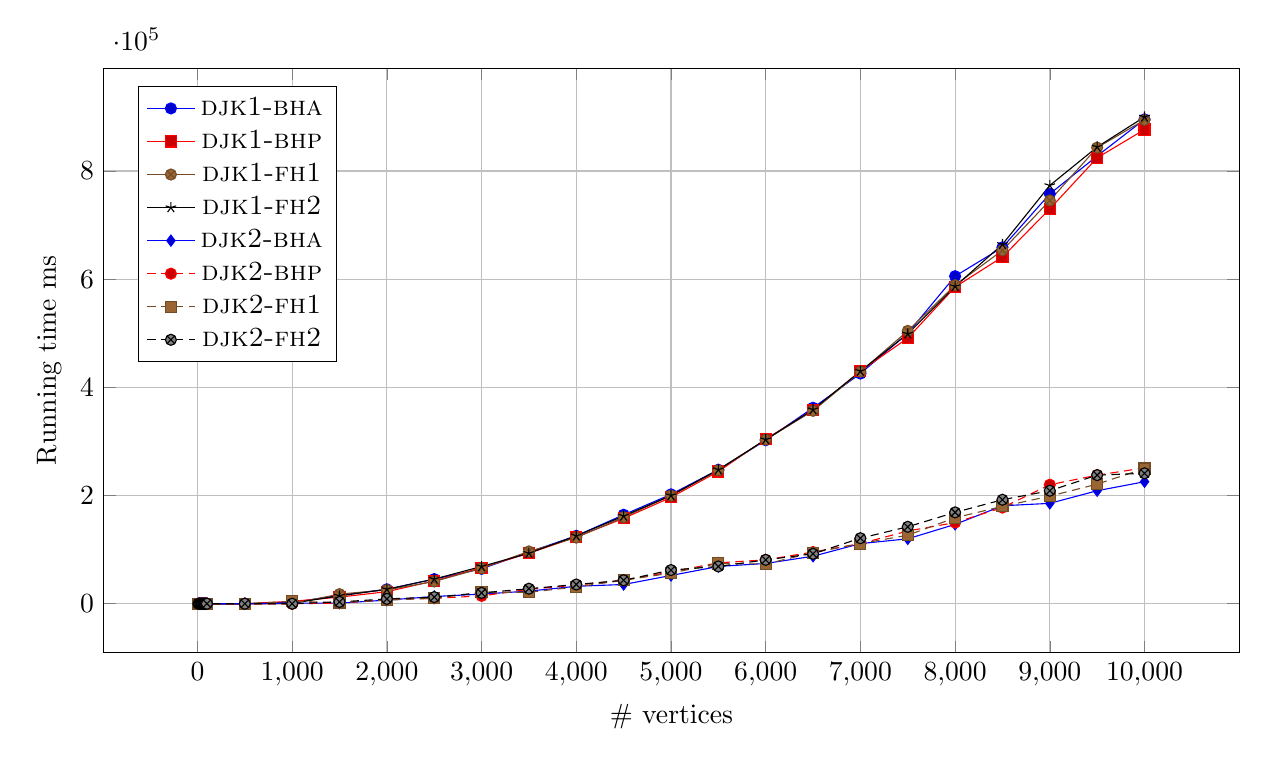
\begin{tikzpicture}
        \begin{axis}[
            xlabel = \# vertices,
            ylabel = Running time ms,
            height=9cm,
            width=16cm,
            grid=major,
            xtick={0,1000,2000,...,10000},
            scaled x ticks = false,
            legend pos=north west
    	]
    		
    		
    	\addplot coordinates {
(10,0)
(20,0)
(30,0)
(40,0)
(50,0)
(60,0)
(70,0)
(80,0)
(90,0)
(100,0)
(500,0)
(1000,2222)
(1500,15555)
(2000,26666)
(2500,45555)
(3000,64444)
(3500,95555)
(4000,125555)
(4500,164444)
(5000,202222)
(5500,247777)
(6000,302222)
(6500,362222)
(7000,425555)
(7500,500000)
(8000,605555)
(8500,658888)
(9000,757777)
(9500,827777)
(10000,895555)

    	};
        
    	\addlegendentry{\textsc{djk1-bha}}

                \addplot coordinates {
(10,0)
(20,0)
(30,0)
(40,0)
(50,0)
(60,0)
(70,0)
(80,0)
(90,0)
(100,0)
(500,0)
(1000,4444)
(1500,12222)
(2000,22222)
(2500,42222)
(3000,66666)
(3500,93333)
(4000,123333)
(4500,157777)
(5000,196666)
(5500,244444)
(6000,304444)
(6500,357777)
(7000,430000)
(7500,491111)
(8000,585555)
(8500,641111)
(9000,730000)
(9500,824444)
(10000,876666)

    	};
        
    	\addlegendentry{\textsc{djk1-bhp}}

        \addplot coordinates {
(10,0)
(20,0)
(30,0)
(40,0)
(50,0)
(60,0)
(70,0)
(80,0)
(90,0)
(100,0)
(500,0)
(1000,0)
(1500,17777)
(2000,25555)
(2500,41111)
(3000,65555)
(3500,96666)
(4000,122222)
(4500,160000)
(5000,200000)
(5500,246666)
(6000,303333)
(6500,356666)
(7000,428888)
(7500,504444)
(8000,588888)
(8500,653333)
(9000,745555)
(9500,843333)
(10000,894444)

    	};
        
    	\addlegendentry{\textsc{djk1-fh1}}

        \addplot coordinates {
(10,0)
(20,0)
(30,0)
(40,0)
(50,0)
(60,0)
(70,0)
(80,0)
(90,0)
(100,0)
(500,0)
(1000,1111)
(1500,14444)
(2000,26666)
(2500,45555)
(3000,68888)
(3500,93333)
(4000,125555)
(4500,162222)
(5000,200000)
(5500,247777)
(6000,303333)
(6500,358888)
(7000,430000)
(7500,498888)
(8000,586666)
(8500,664444)
(9000,773333)
(9500,844444)
(10000,900000)

    	};
        
    	\addlegendentry{\textsc{djk1-fh2}}


        \addplot coordinates {
(10,0)
(20,0)
(30,0)
(40,0)
(50,0)
(60,0)
(70,0)
(80,0)
(90,0)
(100,0)
(500,0)
(1000,1111)
(1500,1111)
(2000,6666)
(2500,13333)
(3000,17777)
(3500,23333)
(4000,32222)
(4500,35555)
(5000,52222)
(5500,68888)
(6000,74444)
(6500,87777)
(7000,111111)
(7500,120000)
(8000,146666)
(8500,181111)
(9000,185555)
(9500,208888)
(10000,225555)
        };
        
    	\addlegendentry{\textsc{djk2-bha}}

        \addplot coordinates {
(10,0)
(20,0)
(30,0)
(40,0)
(50,0)
(60,0)
(70,0)
(80,0)
(90,0)
(100,0)
(500,0)
(1000,0)
(1500,1111)
(2000,7777)
(2500,10000)
(3000,14444)
(3500,26666)
(4000,34444)
(4500,43333)
(5000,58888)
(5500,75555)
(6000,81111)
(6500,95555)
(7000,111111)
(7500,134444)
(8000,150000)
(8500,177777)
(9000,220000)
(9500,237777)
(10000,251111)
        };
        
        \addlegendentry{\textsc{djk2-bhp}}

        \addplot coordinates {
(10,0)
(20,0)
(30,0)
(40,0)
(50,0)
(60,0)
(70,0)
(80,0)
(90,0)
(100,0)
(500,0)
(1000,4444)
(1500,2222)
(2000,6666)
(2500,10000)
(3000,21111)
(3500,21111)
(4000,31111)
(4500,43333)
(5000,56666)
(5500,74444)
(6000,73333)
(6500,94444)
(7000,111111)
(7500,126666)
(8000,158888)
(8500,180000)
(9000,198888)
(9500,221111)
(10000,250000)
        };
        
        \addlegendentry{\textsc{djk2-fh1}}
        
        \addplot coordinates {
(10,0)
(20,0)
(30,0)
(40,0)
(50,0)
(60,0)
(70,0)
(80,0)
(90,0)
(100,0)
(500,0)
(1000,0)
(1500,3333)
(2000,8888)
(2500,12222)
(3000,20000)
(3500,27777)
(4000,35555)
(4500,43333)
(5000,62222)
(5500,68888)
(6000,81111)
(6500,92222)
(7000,121111)
(7500,142222)
(8000,168888)
(8500,192222)
(9000,208888)
(9500,237777)
(10000,241111)
        };
        
        \addlegendentry{\textsc{djk2-fh2}}

        \end{axis}

    \end{tikzpicture}
    \captionof{figure}{Average time of running \textsc{Dijkstra1} and \textsc{Dijkstra2} on 20 \% connected graph}
    \label{fig:sample_figure}
\end{minipage}

\begin{minipage}[c]{\textwidth}
\centering
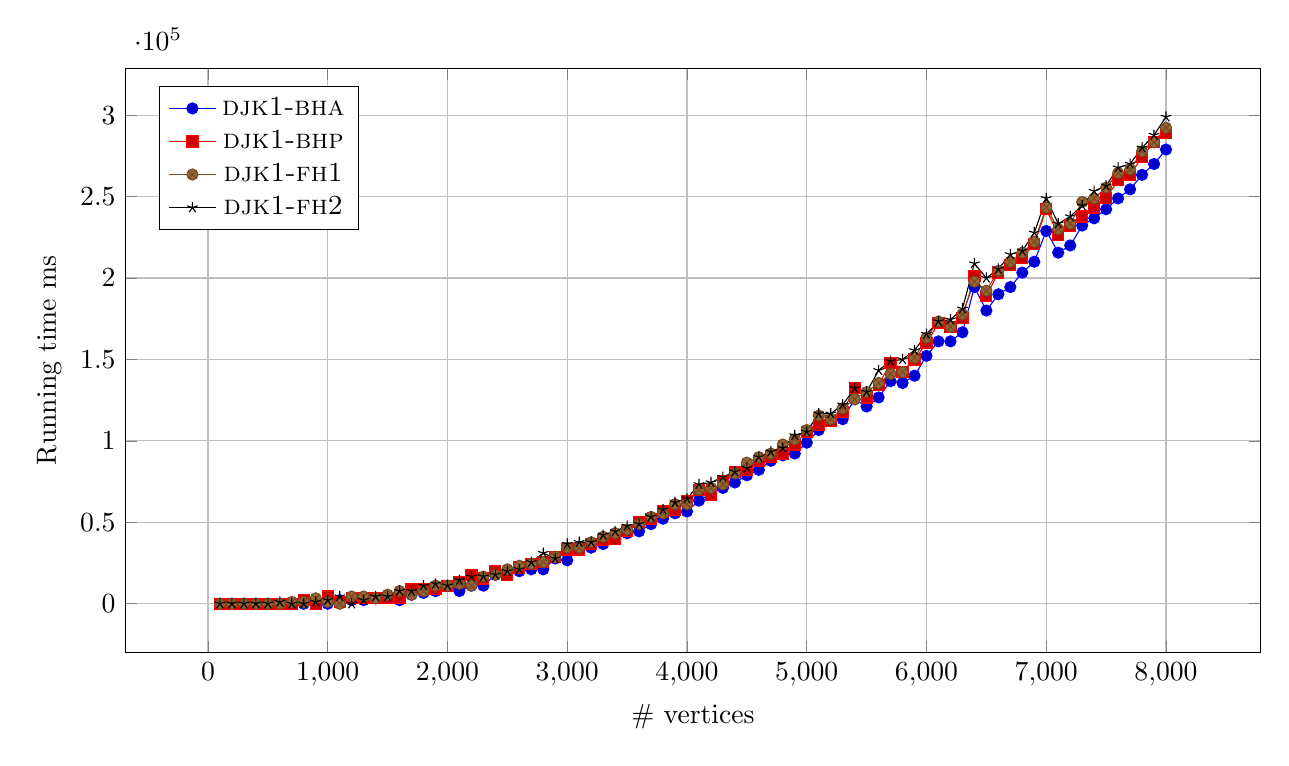
\begin{tikzpicture}
        \begin{axis}[
            xlabel = \# vertices,
            ylabel = Running time ms,
            height=9cm,
            width=16cm,
            grid=major,
            legend pos=north west
    	]
    		
    	\addplot coordinates {
(100,0)
(200,0)
(300,0)
(400,0)
(500,0)
(600,0)
(700,0)
(800,0)
(900,1111)
(1000,0)
(1100,2222)
(1200,2222)
(1300,2222)
(1400,3333)
(1500,4444)
(1600,2222)
(1700,5555)
(1800,6666)
(1900,7777)
(2000,11111)
(2100,7777)
(2200,11111)
(2300,11111)
(2400,17777)
(2500,20000)
(2600,20000)
(2700,21111)
(2800,21111)
(2900,27777)
(3000,26666)
(3100,33333)
(3200,34444)
(3300,36666)
(3400,40000)
(3500,43333)
(3600,44444)
(3700,48888)
(3800,52222)
(3900,55555)
(4000,56666)
(4100,63333)
(4200,67777)
(4300,71111)
(4400,74444)
(4500,78888)
(4600,82222)
(4700,87777)
(4800,91111)
(4900,92222)
(5000,98888)
(5100,106666)
(5200,112222)
(5300,113333)
(5400,125555)
(5500,121111)
(5600,126666)
(5700,136666)
(5800,135555)
(5900,140000)
(6000,152222)
(6100,161111)
(6200,161111)
(6300,166666)
(6400,194444)
(6500,180000)
(6600,190000)
(6700,194444)
(6800,203333)
(6900,210000)
(7000,228888)
(7100,215555)
(7200,220000)
(7300,232222)
(7400,236666)
(7500,242222)
(7600,248888)
(7700,254444)
(7800,263333)
(7900,270000)
(8000,278888)
    	};
        
    	\addlegendentry{\textsc{djk1-bha}}

                \addplot coordinates {
(100,0)
(200,0)
(300,0)
(400,0)
(500,0)
(600,0)
(700,0)
(800,2222)
(900,0)
(1000,4444)
(1100,1111)
(1200,3333)
(1300,3333)
(1400,3333)
(1500,3333)
(1600,3333)
(1700,8888)
(1800,8888)
(1900,8888)
(2000,11111)
(2100,13333)
(2200,17777)
(2300,15555)
(2400,20000)
(2500,17777)
(2600,22222)
(2700,24444)
(2800,25555)
(2900,28888)
(3000,33333)
(3100,33333)
(3200,36666)
(3300,38888)
(3400,40000)
(3500,44444)
(3600,50000)
(3700,52222)
(3800,56666)
(3900,57777)
(4000,63333)
(4100,70000)
(4200,66666)
(4300,75555)
(4400,81111)
(4500,82222)
(4600,87777)
(4700,90000)
(4800,92222)
(4900,97777)
(5000,105555)
(5100,110000)
(5200,112222)
(5300,117777)
(5400,132222)
(5500,126666)
(5600,134444)
(5700,147777)
(5800,142222)
(5900,150000)
(6000,160000)
(6100,172222)
(6200,170000)
(6300,175555)
(6400,201111)
(6500,188888)
(6600,203333)
(6700,207777)
(6800,212222)
(6900,221111)
(7000,242222)
(7100,226666)
(7200,232222)
(7300,237777)
(7400,243333)
(7500,248888)
(7600,260000)
(7700,263333)
(7800,274444)
(7900,283333)
(8000,288888)
    	};
        
    	\addlegendentry{\textsc{djk1-bhp}}

        \addplot coordinates {
(100,0)
(200,0)
(300,0)
(400,0)
(500,0)
(600,0)
(700,1111)
(800,1111)
(900,3333)
(1000,1111)
(1100,0)
(1200,4444)
(1300,4444)
(1400,3333)
(1500,5555)
(1600,7777)
(1700,5555)
(1800,7777)
(1900,11111)
(2000,11111)
(2100,12222)
(2200,11111)
(2300,16666)
(2400,17777)
(2500,21111)
(2600,23333)
(2700,24444)
(2800,25555)
(2900,28888)
(3000,34444)
(3100,34444)
(3200,37777)
(3300,41111)
(3400,43333)
(3500,45555)
(3600,48888)
(3700,53333)
(3800,55555)
(3900,61111)
(4000,61111)
(4100,70000)
(4200,71111)
(4300,73333)
(4400,80000)
(4500,86666)
(4600,90000)
(4700,92222)
(4800,97777)
(4900,101111)
(5000,106666)
(5100,115555)
(5200,113333)
(5300,120000)
(5400,125555)
(5500,130000)
(5600,135555)
(5700,141111)
(5800,142222)
(5900,151111)
(6000,163333)
(6100,173333)
(6200,170000)
(6300,177777)
(6400,197777)
(6500,192222)
(6600,204444)
(6700,210000)
(6800,215555)
(6900,222222)
(7000,243333)
(7100,230000)
(7200,233333)
(7300,246666)
(7400,248888)
(7500,255555)
(7600,264444)
(7700,266666)
(7800,277777)
(7900,283333)
(8000,292222)
    	};
        
    	\addlegendentry{\textsc{djk1-fh1}}

        \addplot coordinates {
(100,0)
(200,0)
(300,0)
(400,0)
(500,0)
(600,1111)
(700,0)
(800,0)
(900,1111)
(1000,2222)
(1100,4444)
(1200,0)
(1300,2222)
(1400,4444)
(1500,4444)
(1600,7777)
(1700,7777)
(1800,11111)
(1900,12222)
(2000,11111)
(2100,14444)
(2200,16666)
(2300,16666)
(2400,17777)
(2500,20000)
(2600,21111)
(2700,25555)
(2800,31111)
(2900,27777)
(3000,36666)
(3100,37777)
(3200,37777)
(3300,42222)
(3400,44444)
(3500,47777)
(3600,48888)
(3700,53333)
(3800,57777)
(3900,62222)
(4000,64444)
(4100,73333)
(4200,74444)
(4300,77777)
(4400,81111)
(4500,83333)
(4600,90000)
(4700,93333)
(4800,95555)
(4900,103333)
(5000,105555)
(5100,116666)
(5200,116666)
(5300,122222)
(5400,132222)
(5500,130000)
(5600,143333)
(5700,148888)
(5800,150000)
(5900,155555)
(6000,165555)
(6100,173333)
(6200,174444)
(6300,181111)
(6400,208888)
(6500,200000)
(6600,205555)
(6700,214444)
(6800,216666)
(6900,227777)
(7000,248888)
(7100,233333)
(7200,237777)
(7300,244444)
(7400,253333)
(7500,256666)
(7600,267777)
(7700,270000)
(7800,280000)
(7900,287777)
(8000,298888)
    	};
        
    	\addlegendentry{\textsc{djk1-fh2}}


        \addplot coordinates {
        };
        
    	\addlegendentry{\textsc{djk2-bha}}

        \addplot coordinates {
        };
        
        \addlegendentry{\textsc{djk2-bhp}}

        \addplot coordinates {
        };
        
        \addlegendentry{\textsc{djk2-fh1}}
        
        \addplot coordinates {
        };
        
        \addlegendentry{\textsc{djk2-fh2}}

        \end{axis}

    \end{tikzpicture}
    \captionof{figure}{Average time of running \textsc{Dijkstra1} and \textsc{Dijkstra2} on 10 \% connected graph}
    \label{fig:sample_figure}
\end{minipage}


\chapter{Conlusion}

needs contents


%%%%%%%%%%%%%%%%%%%%%%%%%%%%%%%%%%%%%%%%%%%%%%%%%%%%%%%%%%%%%%%%%%%%%%%

\addcontentsline{toc}{chapter}{Bibliography}
\bibliographystyle{plain} 
\bibliography{report}

\end{document}

